\chapter{ผลการดำเนินงาน}

ดำเนินงานของโปรเจคนี้จะแบ่งออกมาเป็นทั้งหมด 3 ส่วน โดยส่วนแรกคือส่วนของการจัดเก็บข้อมูลเข้าสู่ระบบโดยนำรูปภาพได้ที่ได้รับมาผ่านกระบวนการ Image Processing ก่อนจะนำไปผ่านกระบวนการ OCR และ Text Processing ก่อนจะถูกเก็บข้อมูลในระบบ ส่วนที่สองการค้นหาข้อมูล เป็นการค้นหาแบบ IR (Information retrieval) โดยนำคะแนน TF-IDF มาใช้เป็นคะแนนในการค้นหา และส่วนสุดท้ายคือส่วนของการทำแพลตฟอร์มเว็ปไซต์

\section{ผลลัพธ์ที่ได้จากการทำ Image processing}

\subsection{เปรียบเทียบประสิทธิภาพในการทำ OCR ของ การทำ Image process แต่ละแบบ}

จากการทดสอบประสิทธิภาพของการทำ image processing ทั้งสองแบบพบว่า การทำ image process แบบแรกนั้นมีคำผิดน้อยกว่า แต่มีคำที่ไม่ถูกอ่านมากถึง 32.71\% ดังตารางที่ \ref{tbl:imagep1} ซึ่งต่างจากการทำ image process แบบที่ 2 ที่่ค่าความถูกต้องของคำมี 74.74 \% ดังตาราง \ref{tbl:imagep2}

\subsubsection{แบบที่ 1 การใช้ Skip page , Rotated, remove picture, remove line และ group text}
\begin{table}[H]
    \caption{ตารางประเมินการทำ image processing แบบที่ 1 }\label{tbl:imagep1}
    \begin{tabular}{|c|c|c|c|c|c|c|c|}
        \hline
        หนังสือ                             & หน้า  & คำทั้งหมด & คำผิดที่เจอ & \%    & คำเกิน & คำที่ไม่โดนอ่าน & \%    \\ \hline
        \multirow{2}{*}{กตเวทิตาปี 2542}    & 15    & 4         & 4           & 100 \%  & 0      & 0               & 0 \%    \\ \cline{2-8} 
                                            & 29    & 252       & 14          & 5.56 \%  & 46     & 2               & 0.79 \% \\ \hline
        \multirow{2}{*}{กตเวทิตาปี 2556}    & 15    & 242       & 33          & 13.64 \% & 2      & 1               & 0.41 \% \\ \cline{2-8} 
                                            & 29    & 257       & 20          & 7.78 \% & 3      & 10              & 3.89 \% \\ \hline
        \multirow{2}{*}{รายงานประจำปี 2544} & 15    & 47        & 3           & 6.38 \% & 2      & 34              & 72.34 \% \\ \cline{2-8} 
                                            & 29    & 585       & 39          & 6.67 \% & 3      & 308             & 52.65 \% \\ \hline
        \multirow{2}{*}{รายงานประจำปี 2553} & 15    & 68        & 0           & 0 \%    & 0      & 68              & 100 \%  \\ \cline{2-8} 
                                            & 29    & 596       & 17          & 2.85 \% & 8      & 340             & 57.05 \% \\ \hline
        \multirow{2}{*}{รายงานประจำปี 2549} & 15    & 155       & 53          & 34.19 \% & 42     & 45              & 29.03 \% \\ \cline{2-8} 
                                            & 29    & 304       & 22          & 7.24 \% & 20     & 13              & 4.28 \%\\ \hline
        \multicolumn{1}{|l|}{}              & total & 2510      & 205         & 8.17 \% & 126    & 821             & 32.71 \% \\ \hline
        \end{tabular}
        \end{table}

\subsubsection{แบบที่ 2 ใช้การ Remove Background}

\begin{table}[H]
    \caption{ตารางประเมินการทำ image processing แบบที่ 2}\label{tbl:imagep2}
        \begin{tabular}{|c|c|c|c|c|c|c|c|}
            \hline
            หนังสือ                             & หน้า                       & คำทั้งหมด & คำผิดที่เจอ & \%    & คำเกิน & คำที่ไม่โดนอ่าน & \%    \\ \hline
            \multirow{2}{*}{กตเวทิตาปี 2542}    & 15                         & 4         & 4           & 100\%   & 0      & 0               & 0\%     \\ \cline{2-8} 
                                                & 29                         & 252       & 30          & 11.9\%  & 6      & 9               & 3.57\%  \\ \hline
            \multirow{2}{*}{กตเวทิตาปี 2556}    & 15                         & 242       & 42          & 17.36\% & 2      & 48              & 19.83\% \\ \cline{2-8} 
                                                & 29                         & 257       & 54          & 21.01\% & 2      & 62              & 24.12\% \\ \hline
            \multirow{2}{*}{รายงานประจำปี 2544} & 15                         & 47        & 27          & 57.45\% & 5      & 5               & 10.64\% \\ \cline{2-8} 
                                                & 29                         & 585       & 101         & 17.26\% & 23     & 0               & 0\%     \\ \hline
            \multirow{2}{*}{รายงานประจำปี 2553} & 15                         & 68        & 30          & 44.12\% & 7      & 0               & 0\%     \\ \cline{2-8} 
                                                & 29                         & 596       & 85          & 14.26\% & 30     & 0               & 0\%     \\ \hline
            \multirow{2}{*}{รายงานประจำปี 2549} & 15                         & 155       & 57          & 36.77\% & 14     & 4               & 2.58\%  \\ \cline{2-8} 
                                                & 29                         & 304       & 76          & 25\%    & 7      & 0               & 0\%     \\ \hline
            \multicolumn{1}{|l|}{}              & \multicolumn{1}{l|}{total} & 2510      & 506         & 20.16\% & 96     & 128             & 5.1\%   \\ \hline
            \end{tabular}
            \end{table}

\section{ผลการเปรียบเทียบข้อมูล 2 ชุด}

\begin{table}[H]
    \caption{ตารางประเมินข้อมูลชุดที่ 1}\label{tbl:bigdata}
        \begin{tabular}{|c|c|c|c|c|c|c|c|}
            \hline
            หนังสือ                             & หน้า  & คำทั้งหมด & คำผิดที่เจอ & \%    & คำเกิน & คำที่ไม่โดนอ่าน & \%    \\ \hline
            \multirow{2}{*}{กตเวทิตาปี 2542}    & 15    & 4         & 2           & 50\%    & 0      & 2               & 50\%    \\ \cline{2-8} 
                                                & 29    & 252       & 34          & 13.49\% & 12     & 4               & 1.59\%  \\ \hline
            \multirow{2}{*}{กตเวทิตาปี 2556}    & 15    & 242       & 37          & 15.29\% & 0      & 49              & 20.25\% \\ \cline{2-8} 
                                                & 29    & 257       & 47          & 18.29\% & 2      & 45              & 17.51\% \\ \hline
            \multirow{2}{*}{รายงานประจำปี 2544} & 15    & 47        & 40          & 85.11\% & 0      & 4               & 8.51\%  \\ \cline{2-8} 
                                                & 29    & 585       & 78          & 13.33\% & 11     & 15              & 2.56\%  \\ \hline
            \multirow{2}{*}{รายงานประจำปี 2553} & 15    & 68        & 44          & 64.71\% & 0      & 0               & 0\%     \\ \cline{2-8} 
                                                & 29    & 596       & 76          & 12.75\% & 9      & 12              & 2.01\%  \\ \hline
            \multirow{2}{*}{รายงานประจำปี 2549} & 15    & 155       & 44          & 28.39\% & 15     & 1               & 0.65\%  \\ \cline{2-8} 
                                                & 29    & 304       & 53          & 17.43\% & 34     & 0               & 0\%     \\ \hline
                                                & total & 2510      & 455         & 18.13\% & 83     & 132             & 5.26\%  \\ \hline
            \end{tabular}
            \end{table}

\begin{table}[H]
    \caption{ตารางประเมินข้อมูลชุดที่ 2}\label{tbl:smalldata}
    \begin{tabular}{|c|c|c|c|c|c|c|c|}
        \hline
        หนังสือ                             & หน้า  & คำทั้งหมด & คำผิดที่เจอ & \%    & คำเกิน & คำที่ไม่โดนอ่าน & \%    \\ \hline
        \multirow{2}{*}{กตเวทิตาปี 2542}    & 15    & 4         & 4           & 100\%   & 0      & 0               & 0\%     \\ \cline{2-8} 
                                            & 29    & 252       & 40          & 15.87\% & 20     & 10              & 3.97\%  \\ \hline
        \multirow{2}{*}{กตเวทิตาปี 2556}    & 15    & 242       & 46          & 19.01\% & 11     & 44              & 18.18\% \\ \cline{2-8} 
                                            & 29    & 257       & 32          & 12.45\% & 2      & 62              & 24.12\% \\ \hline
        \multirow{2}{*}{รายงานประจำปี 2544} & 15    & 47        & 26          & 55.32\% & 0      & 4               & 8.51\%  \\ \cline{2-8} 
                                            & 29    & 585       & 63          & 10.77\% & 7      & 28              & 4.79\%  \\ \hline
        \multirow{2}{*}{รายงานประจำปี 2553} & 15    & 68        & 36          & 52.94\% & 9      & 2               & 2.94\%  \\ \cline{2-8} 
                                            & 29    & 596       & 65          & 10.91\% & 60     & 2               & 0.34\%  \\ \hline
        \multirow{2}{*}{รายงานประจำปี 2549} & 15    & 155       & 43          & 27.74\% & 30     & 8               & 5.16\%  \\ \cline{2-8} 
                                            & 29    & 304       & 52          & 17.11\% & 34     & 0               & 0\%     \\ \hline
                                            & total & 2510      & 407         & 16.22\% & 173    & 160             & 6.37\%  \\ \hline
        \end{tabular}
        \end{table}

\section{ประสิทธิภาพการแก้ไขคำผิด}
\begin{table}[H]
    \caption{ตารางประเมินข้อมูลชุดที่ 1 ที่ไม่ผ่านการแก้คำผิด}\label{tbl:correction}
    \begin{tabular}{|c|c|c|c|c|c|c|c|}
        \hline
        หนังสือ                             & หน้า                       & คำทั้งหมด & คำผิดที่เจอ & \%    & คำเกิน & คำที่ไม่โดนอ่าน & \%    \\ \hline
        \multirow{2}{*}{กตเวทิตาปี 2542}    & 15                         & 4         & 4           & 100\%   & 0      & 0               & 0\%     \\ \cline{2-8} 
                                            & 29                         & 252       & 30          & 11.9\%  & 6      & 9               & 3.57\%  \\ \hline
        \multirow{2}{*}{กตเวทิตาปี 2556}    & 15                         & 242       & 42          & 17.36\% & 2      & 48              & 19.83\% \\ \cline{2-8} 
                                            & 29                         & 257       & 54          & 21.01\% & 2      & 62              & 24.12\% \\ \hline
        \multirow{2}{*}{รายงานประจำปี 2544} & 15                         & 47        & 27          & 57.45\% & 5      & 5               & 10.64\% \\ \cline{2-8} 
                                            & 29                         & 585       & 101         & 17.26\% & 23     & 0               & 0\%     \\ \hline
        \multirow{2}{*}{รายงานประจำปี 2553} & 15                         & 68        & 30          & 44.12\% & 7      & 0               & 0\%     \\ \cline{2-8} 
                                            & 29                         & 596       & 85          & 14.26\% & 30     & 0               & 0\%     \\ \hline
        \multirow{2}{*}{รายงานประจำปี 2549} & 15                         & 155       & 57          & 36.77\% & 14     & 4               & 2.58\%  \\ \cline{2-8} 
                                            & 29                         & 304       & 76          & 25\%    & 7      & 0               & 0\%     \\ \hline
        \multicolumn{1}{|l|}{}              & \multicolumn{1}{l|}{total} & 2510      & 506         & 20.16\% & 96     & 128             & 5.1\%   \\ \hline
        \end{tabular}
        \end{table}

\begin{table}[H]
    \caption{ตารางประเมินความพึงพอใจ UX-UI design}\label{tbl:uxuieva}
    \begin{tabular}{|p{0.15\linewidth}|p{0.15\linewidth}|p{0.15\linewidth}|p{0.15\linewidth}|p{0.15\linewidth}|c|}
    \hline
                         & \multicolumn{1}{c|}{4}                                                                                                 & \multicolumn{1}{c|}{3}                                                                                   & \multicolumn{1}{c|}{2}                                                                                        & \multicolumn{1}{c|}{1}                                                                        & คะแนนที่ได้ \\ \hline
    ความสมบูรณ์ของข้อมูล    & ข้อมูลมีความสมบูรณ์   ชัดเจนทำให้เข้าใจความหมายที่ต้องการจะสื่อได้เป็นอย่างดี                                          & มีข้อมูลที่ชัดเจน   และแม่นยำในบางครั้ง และสามารถแสดงความหมายที่ต้องการจะสื่อได้บ้าง                     & ข้อมูลมีความแม่นยำ   และชัดเจนบ้าง                                                                            & มีข้อมูลที่ไม่ชัดเจน   ไม่ครบ สื่อความหมายได้ไม่ดี                                            & 3           \\ \hline
    การออกแบบ            & มีการออกแบบที่เน้นความสำคัญและจัดวางองค์ประกอบ   สี เสียง และ animation ได้อย่างเหมาะสม                                & มีการจัดหน้า   และองค์ประกอบทำให้เห็นใจความสำคัญของเนื้อหา มีการใช้ animation   บ้าง                     & การวางหน้าและการจัดองค์ประกอบมีความไม่เหมาะสม   มีการใช้ animation เข้ามาช่วยบ้าง                             & การวางหน้าและการจัดองค์ประกอบมีความไม่เหมาะสมและไม่มีการใช้   animation เข้ามาช่วยในการใช้งาน & 4           \\ \hline
    การใช้งาน              & ผู้ใช้สามารถใช้งานปุ่มหรือย้ายไปยังหน้าต่างๆได้อย่างง่ายดาย   แต่มีลิ้งค์ที่พาไปผิดหน้าอย่างมากหนึ่งลิ้งค์หรือไม่มีเลย & ผู้ใช้สามารถใช้งานปุ่มหรือย้ายไปยังหน้าต่างๆได้อย่างง่ายดาย   แต่มีลิ้งค์ที่พาไปผิดหน้าอย่างมากสองลิ้งค์ & ผู้ใช้มีความสับสนในการใช้ปุ่ม   หรือการย้ายไปยังหน้าต่างๆ บางครั้ง และมีลิ้งค์ที่พาไปผิดหน้าอย่างมากสามลิ้งค์ & ผู้ใช้เกิดความสับสนในปุ่มหรือลิ้งค์ที่ย้ายไปหน้าต่างๆ                                         & 4           \\ \hline
    การใช้ภาษา            & มีการใช้คำผิดหรือภาษาที่ไม่เหมาะสมอย่างมาก   1 จุด                                                                     & มีการใช้คำผิดหรือภาษาที่ไม่เหมาะสมอย่างมาก   2 จุด                                                       & มีการใช้คำผิดหรือภาษาที่ไม่เหมาะสมอย่างมาก 3 จุด                                                              & มีการใช้คำผิดหรือภาษาที่ไม่เหมาะสมมากกว่า 4 จุด                                               & 4           \\ \hline
    \end{tabular}
    \end{table}

\subsection{ผลลัพธ์จากการค้นหา}

ได้มีการออกแบบตารางสำหรับการวัดผลลัพธ์สำหรับการค้นหาทั้งรูปแบบธรรมดาและการใช้โมเดล word2vec เข้ามาช่วยแต่เนื่องจากการล่าช้าจึงทำให้ยังไม่มีการทดสอบผลลัพธ์จากผู้ใช้งานแต่มีการวางแผนว่าเมื่อการค้นหาเสร็จสิ้นจะดำเนินการวัดผลลัพธ์ที่เกิดขึ้นสำหรับการค้นหาว่าตรงตามที่ผู้ใช้ต้องการหรือไม่

\section{ผลลัพธ์ที่ได้จากการเขียนเว็บ}
\subsection{หน้าหลัก}
\begin{figure}[H]
    \centering
    
\includegraphics[scale=0.2]{web1}
    \caption{ภาพแสดงหน้าเว็บหลัก}\label{fig:web1}
\end{figure}

\subsection{การ Authorization เข้าสู่ระบบเว็บไซต์}
\begin{figure}[H]
    \centering
    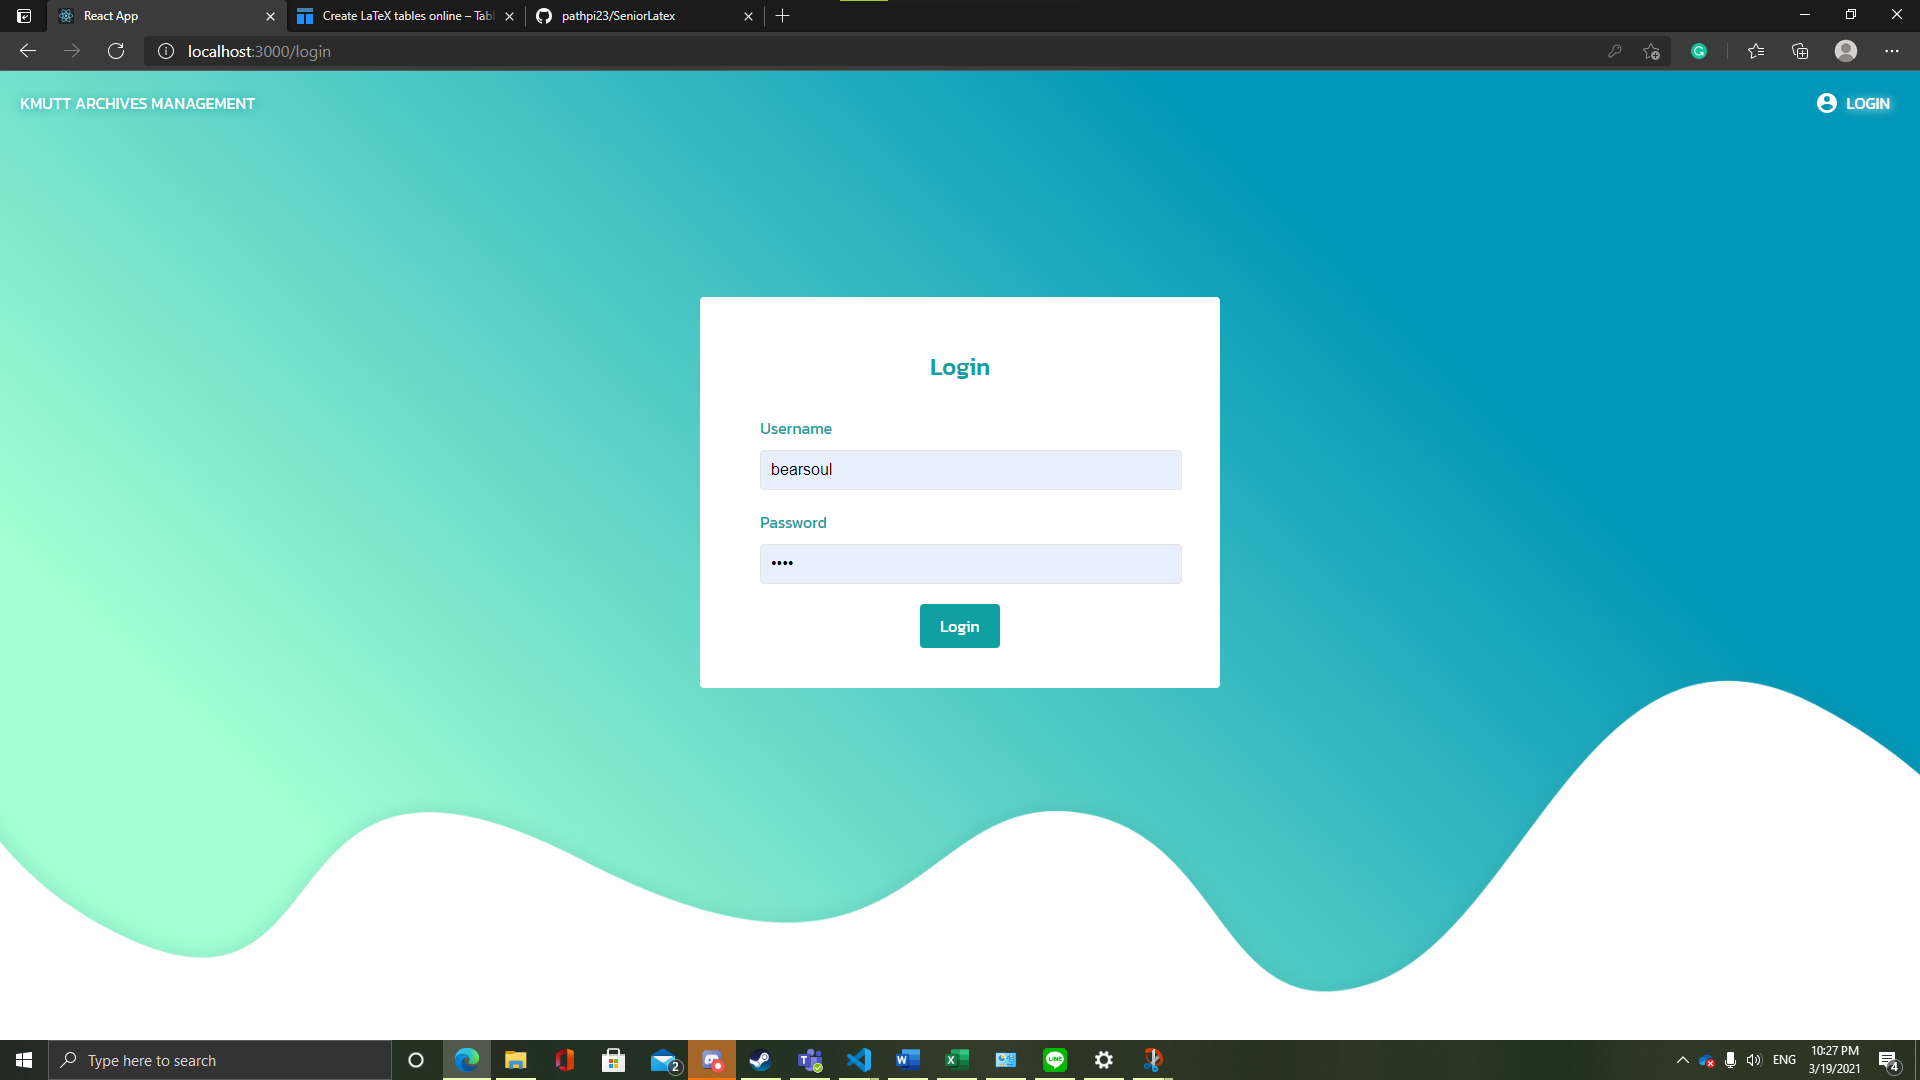
\includegraphics[scale=0.2]{weblogin}
    \caption{ภาพแสดงหน้าเข้าสู่ระบบ}\label{fig:weblogin}
\end{figure}
การเข้าสู่ระบบในเว็บไซต์เราได้ใช้ JSON Web Token (JWT) ในการดูสิทธิ์การเข้าใช้ระบบโดยที่เมื่อผู้ใช้งานเข้าสู่ระบบด้วยรหัสผู้ใช้งานและรหัสผ่านที่ถูกต้องNode JS ก็จะคืน token ที่ถูกเข้ารหัสไว้กลับไปให้ทางเครื่องผู้ใช้งานเก็บใน local storage เพื่อที่จะเป็นการบ่งบอกสิทธิ์การใช้งาน API ที่เหลือทั้งหมดไม่ว่าจะเป็นการค้นหาข้อมูล เพิ่มข้อมูลหนังสือ แก้ไขข้อมูลหนังสือ หรือลบข้อมูลหนังสือออกจากระบบ ถ้าผู้ใช้งานไม่ได้ส่ง token มาด้วยหรือ token นั้นมีการดัดแปลงแก้ไขระบบจะทำการลบ token ภายในเครื่องทึ้งและทำการออกจากระบบโดยทันที

\subsection{การเพิ่มหนังสือเข้าสู่ระบบฐานข้อมูล}
เนื่องจากการเพิ่มหนังสือเข้าสู่ระบบมีขั้นตอนจำนวนมากและใช้เวลานานจึงแบ่งการรอประมวลผลเป็นส่วนของการเพิ่มข้อมูลของหนังสือ ส่วนของการแก้ไขและตรวจสอบคำก่อนนำเข้าสู่ระบบ ส่วนของการตรวจสอบแก้ไข tag ซึ่งผู้ใช้งานไม่จำเป็นต้องรอภายในหน้าเพิ่มหนังสือสามารถไปทำงานฟังก์ชั่นอื่นได้ตามปกติและเมื่อเสร็จกระบวนการเหล่านี้เสร็จจะสามารถกลับมาดำเนินการเพิ่มข้อมูลต่อได้โดยการกดที่หน้า Status และกลับเข้าสู่กระบวนการเพิ่มข้อมูลหนังสือ
\subsubsection{เพิ่มข้อมูลของหนังสือ}
\begin{figure}[H]
    \centering
    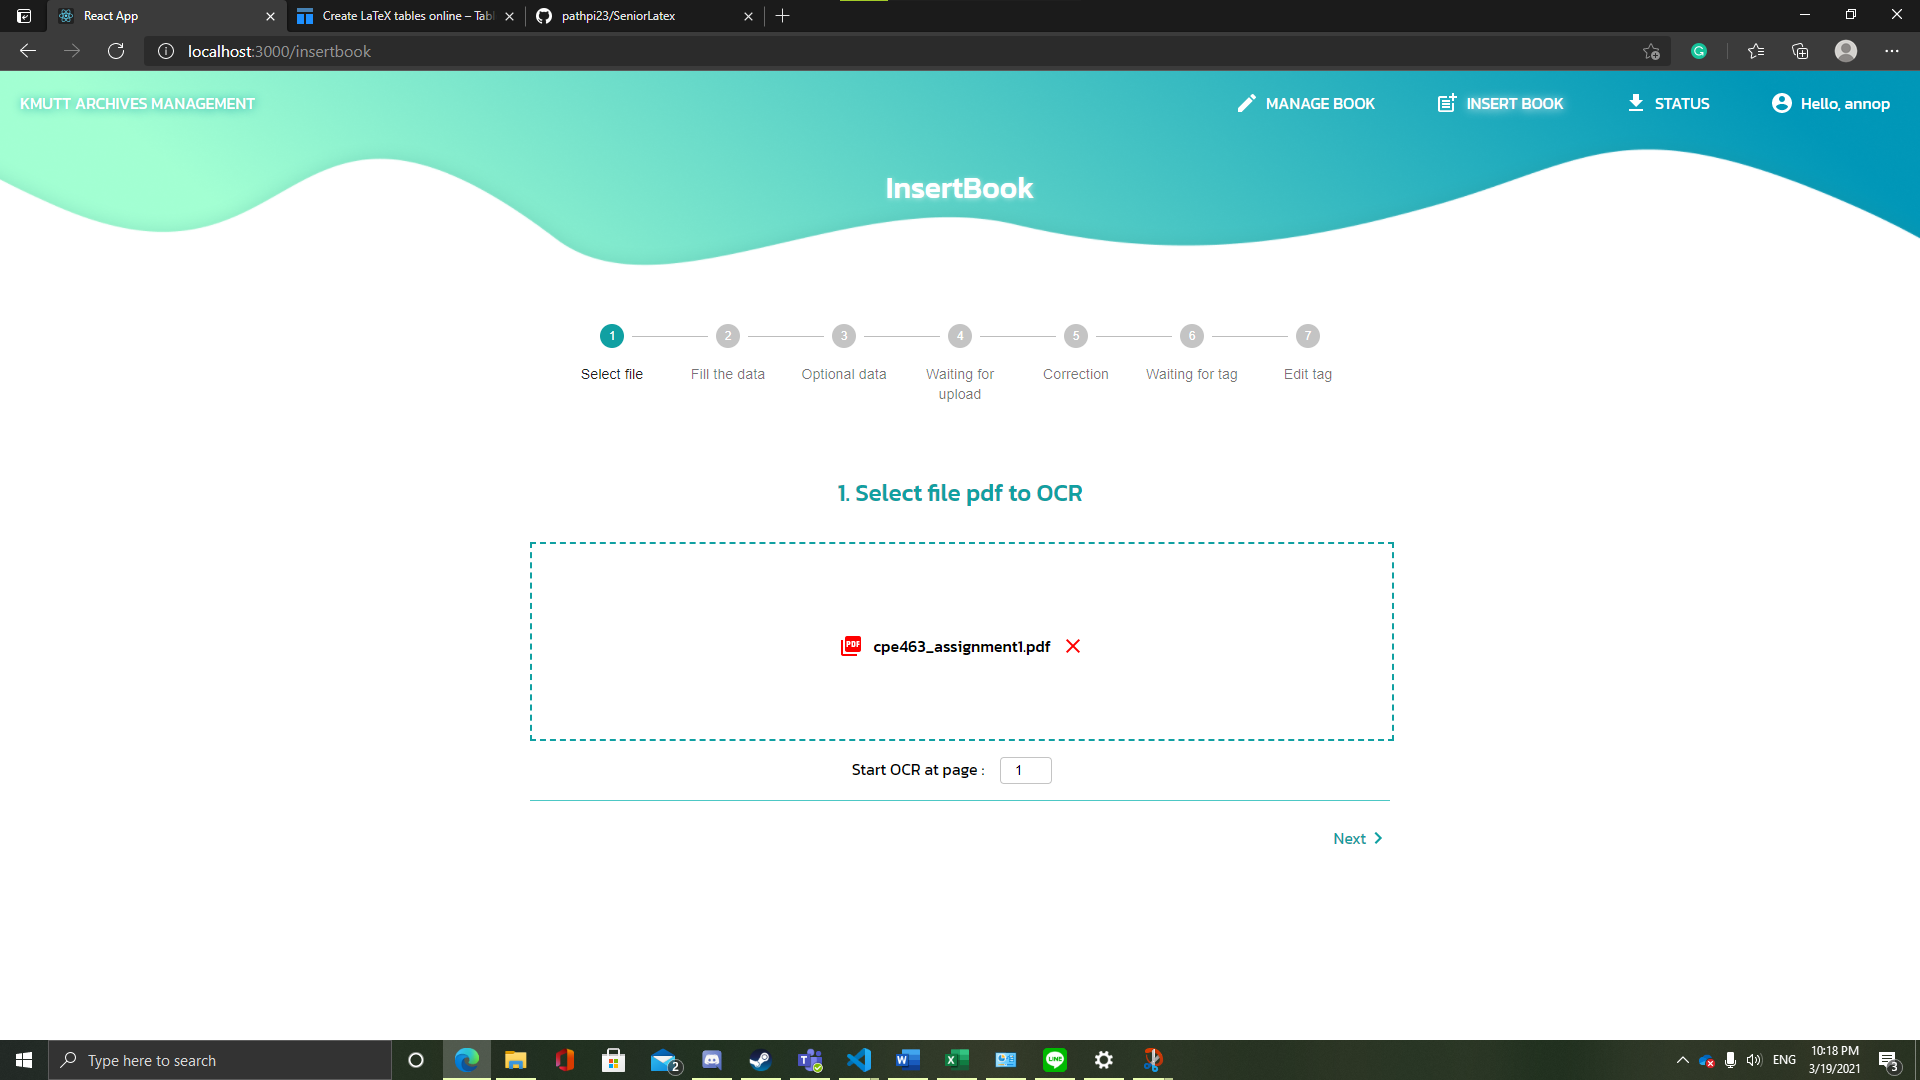
\includegraphics[scale=0.2]{webinsert}
    \caption{ภาพแสดงขั้นตอนการเพิ่มหนังสือขั้นตอนการเพิ่มไฟล์}\label{fig:webinsert}
\end{figure}
\begin{figure}[H]
    \centering
    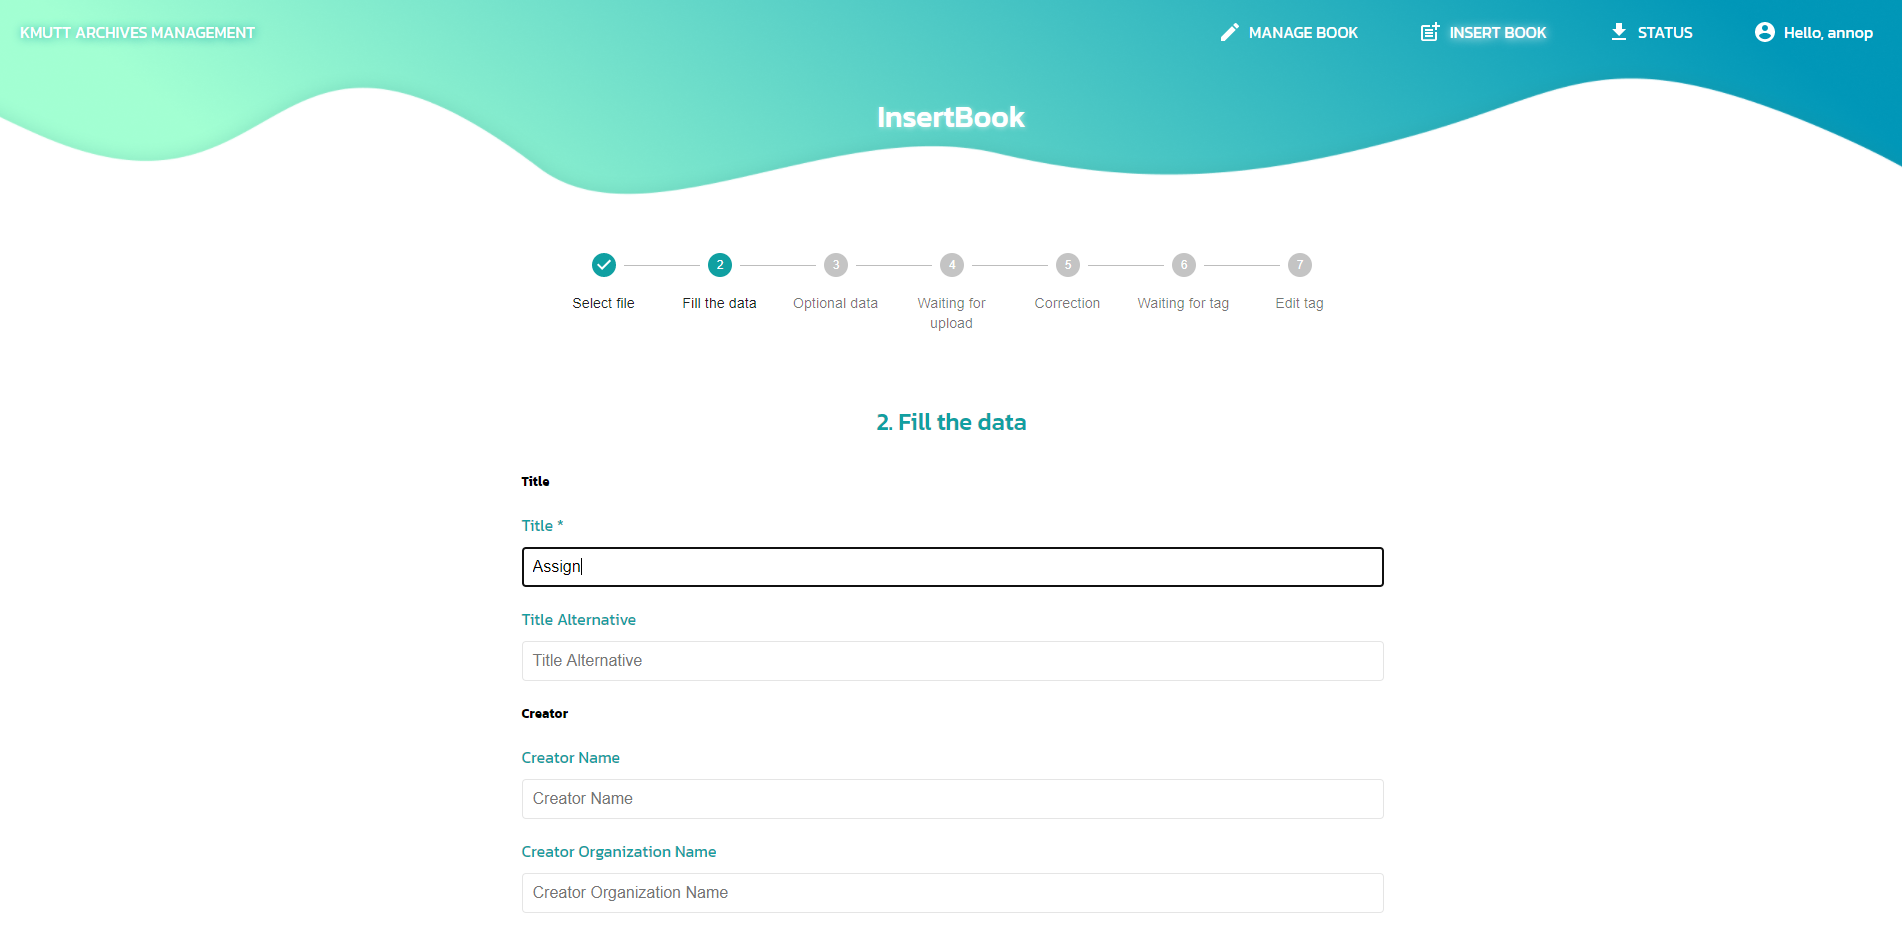
\includegraphics[scale=0.2]{webinsert2}
    \caption{ภาพแสดงขั้นตอนการเพิ่มหนังสือเข้าสู่ระบบขั้นกรอกข้อมูลขั้นที่ 1}\label{fig:webinsert2}
\end{figure}
\begin{figure}[H]
    \centering
    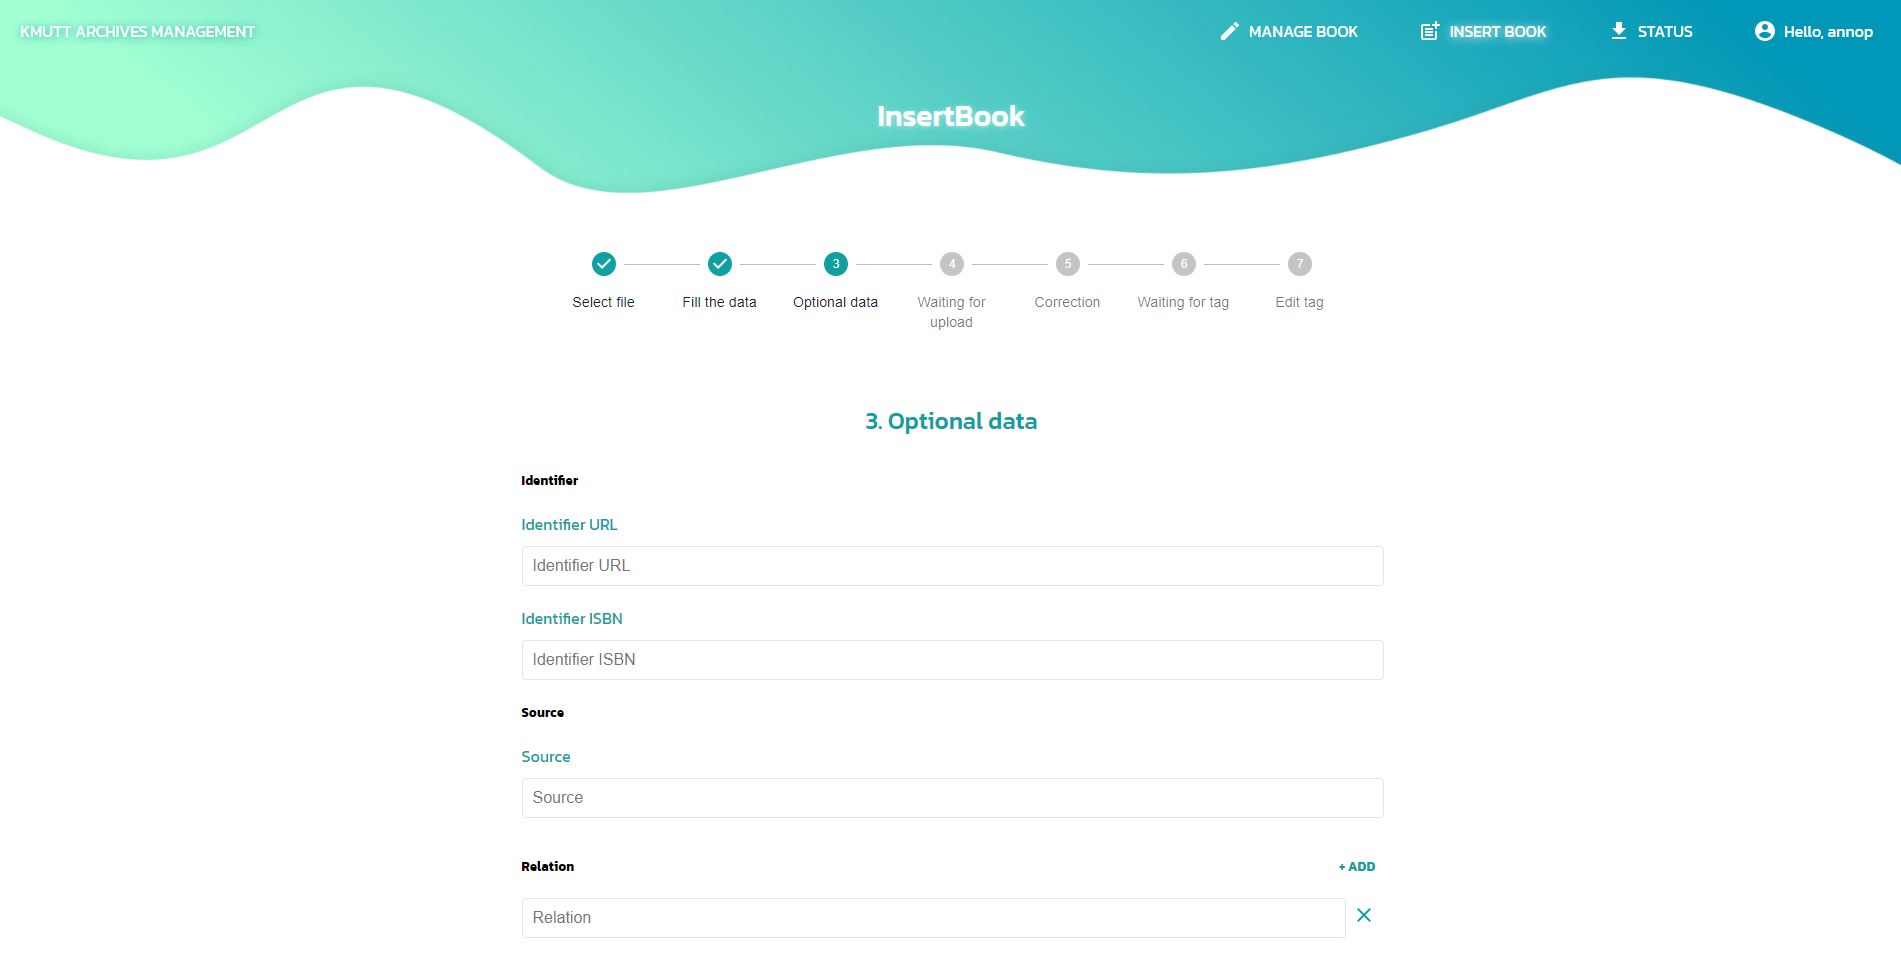
\includegraphics[scale=0.2]{webinsert3}
    \caption{ภาพแสดงขั้นตอนการเพิ่มหนังสือเข้าสู่ระบบขั้นกรอกข้อมูลขั้นที่ 2}\label{fig:webinsert3}
\end{figure}

\begin{figure}[H]
    \centering
    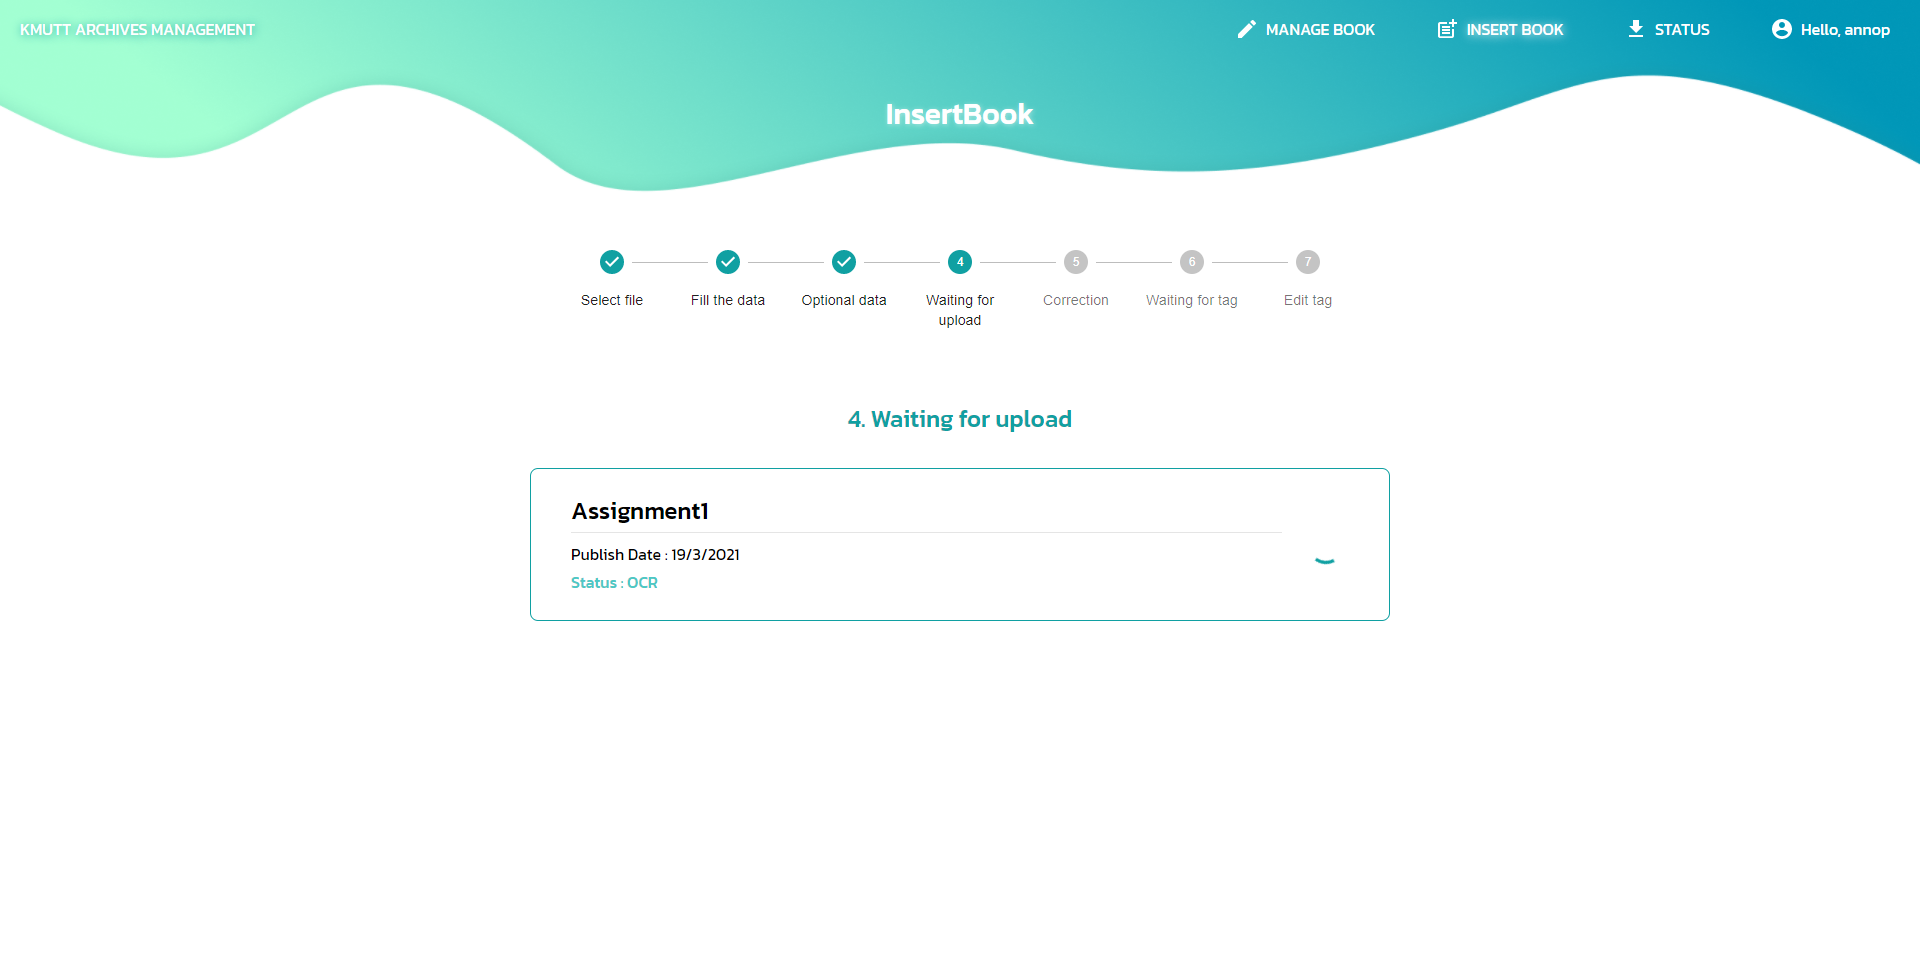
\includegraphics[scale=0.2]{webinsert4}
    \caption{ภาพแสดงขั้นตอนการเพิ่มหนังสือเข้าสู่ระบบขั้นการเตรียมข้อมูล}\label{fig:webdel}
\end{figure}
ในส่วนนี้จะเป็นการใช้ผู้ใช้งานทำการเลือกไฟล์ PDF และกรอกข้อมูลของหนังสือโดยที่เมื่อผู้ใช้งานยืนยันข้อมูลเรียบร้อยแล้วระบบก็จะทำการเพิ่มไฟล์ PDF เพื่อนำไปทำกระบวนการเปลี่ยน PDF เป็นรูปภาพและทำการ OCR และ Text processing  เพื่อทำการแปลงข้อมูลออกมาให้ผู้ใช้งาน

\subsubsection{การแก้ไขและตรวจสอบคำก่อนนำเข้าสู่ระบบ}
\begin{figure}[H]
    \centering
    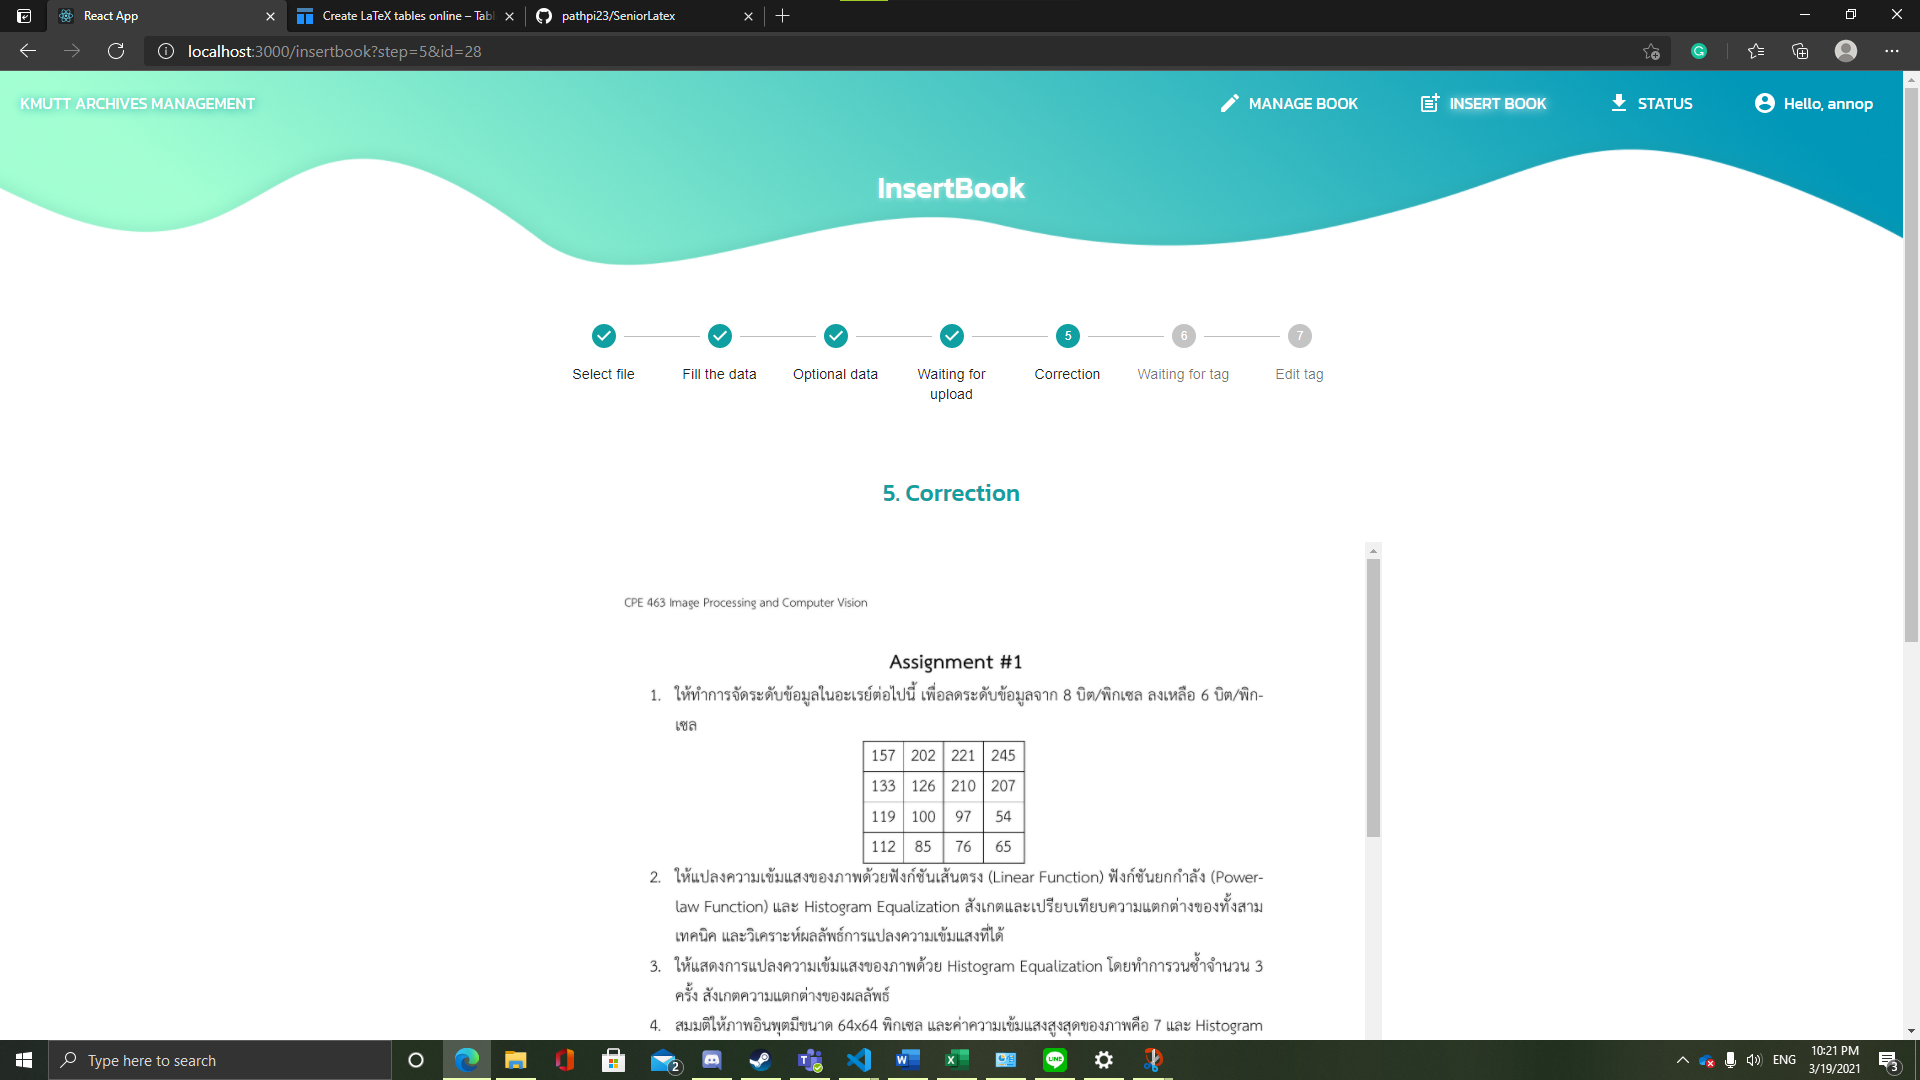
\includegraphics[scale=0.2]{webcorrect}
    \caption{ภาพแสดงขั้นตอนการเพิ่มหนังสือเข้าสู่ระบบขั้นการแก้ไขคำผิด}\label{fig:webcorrect}
\end{figure}

\begin{figure}[H]
    \centering
    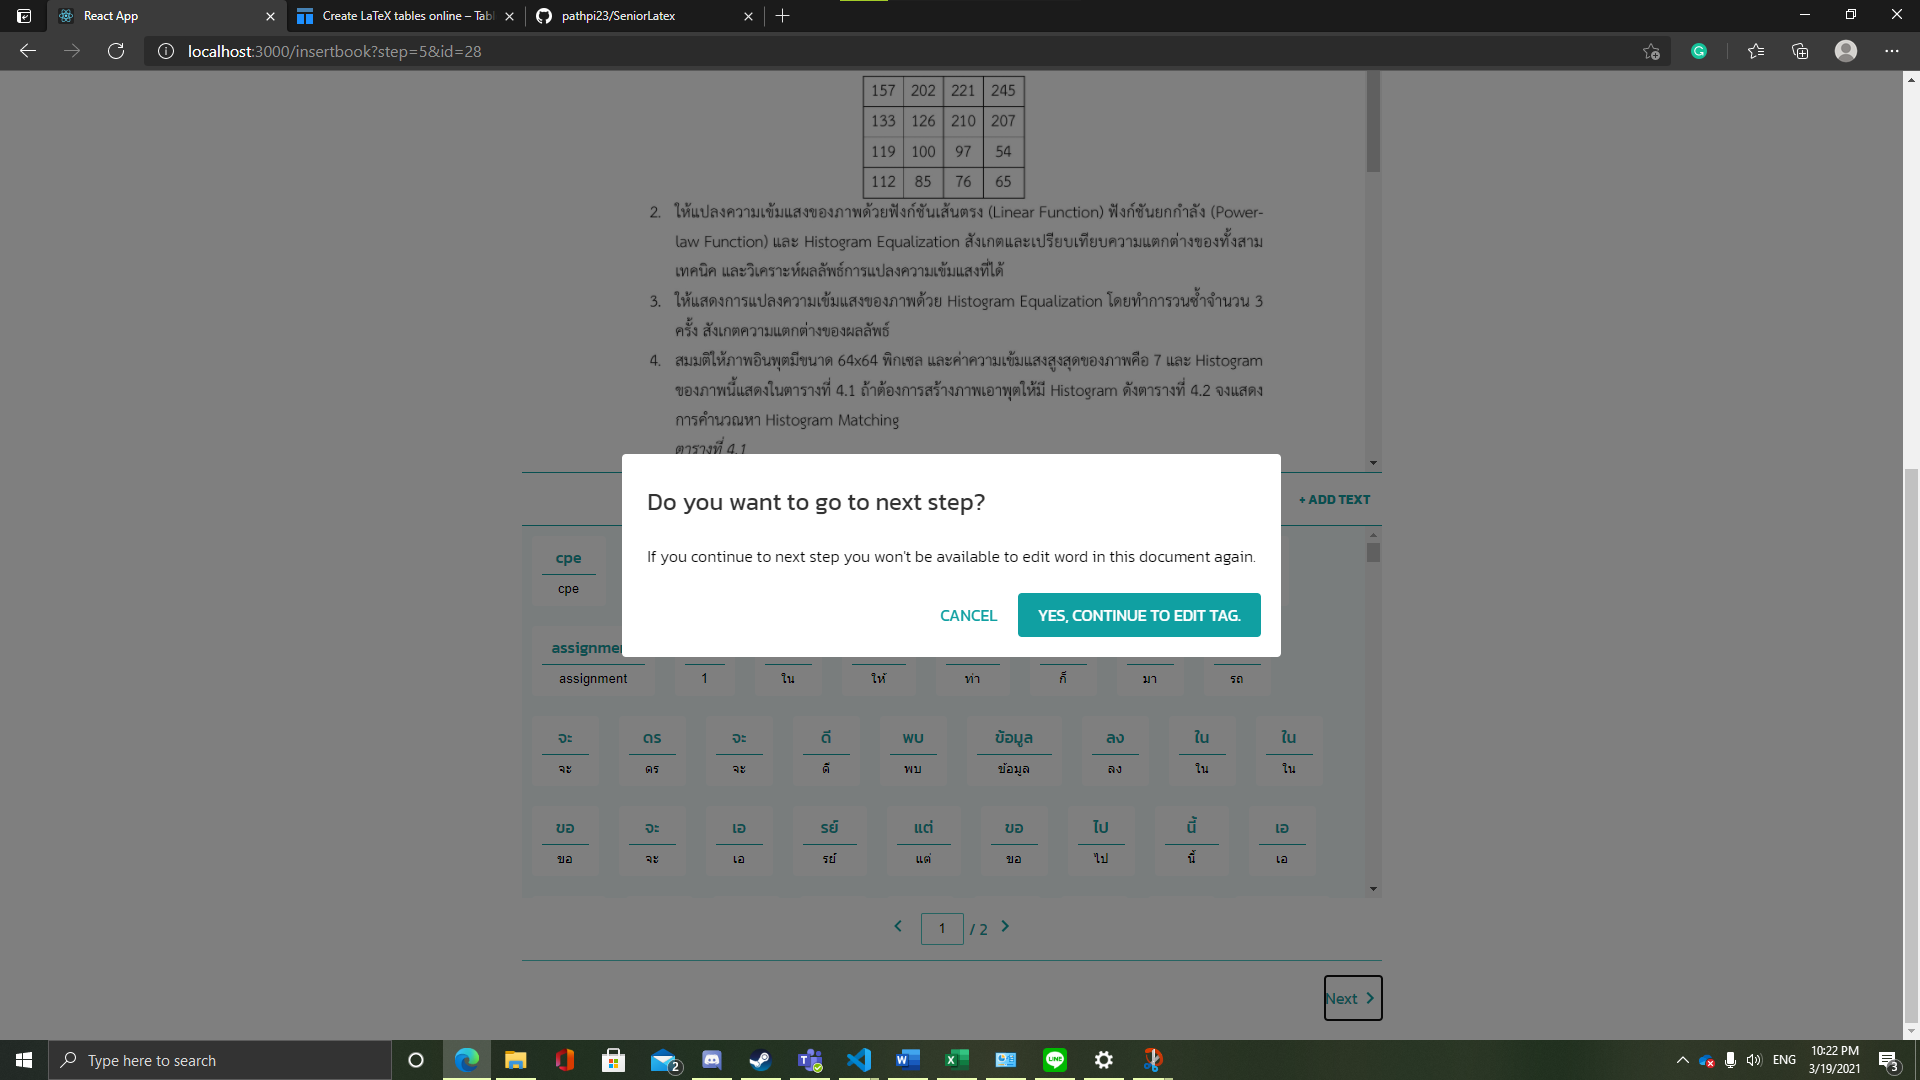
\includegraphics[scale=0.2]{websubmit}
    \caption{ภาพแสดงหน้าต่างยืนยันการแก้คำ}\label{fig:websubmit}
\end{figure}

\begin{figure}[H]
    \centering
    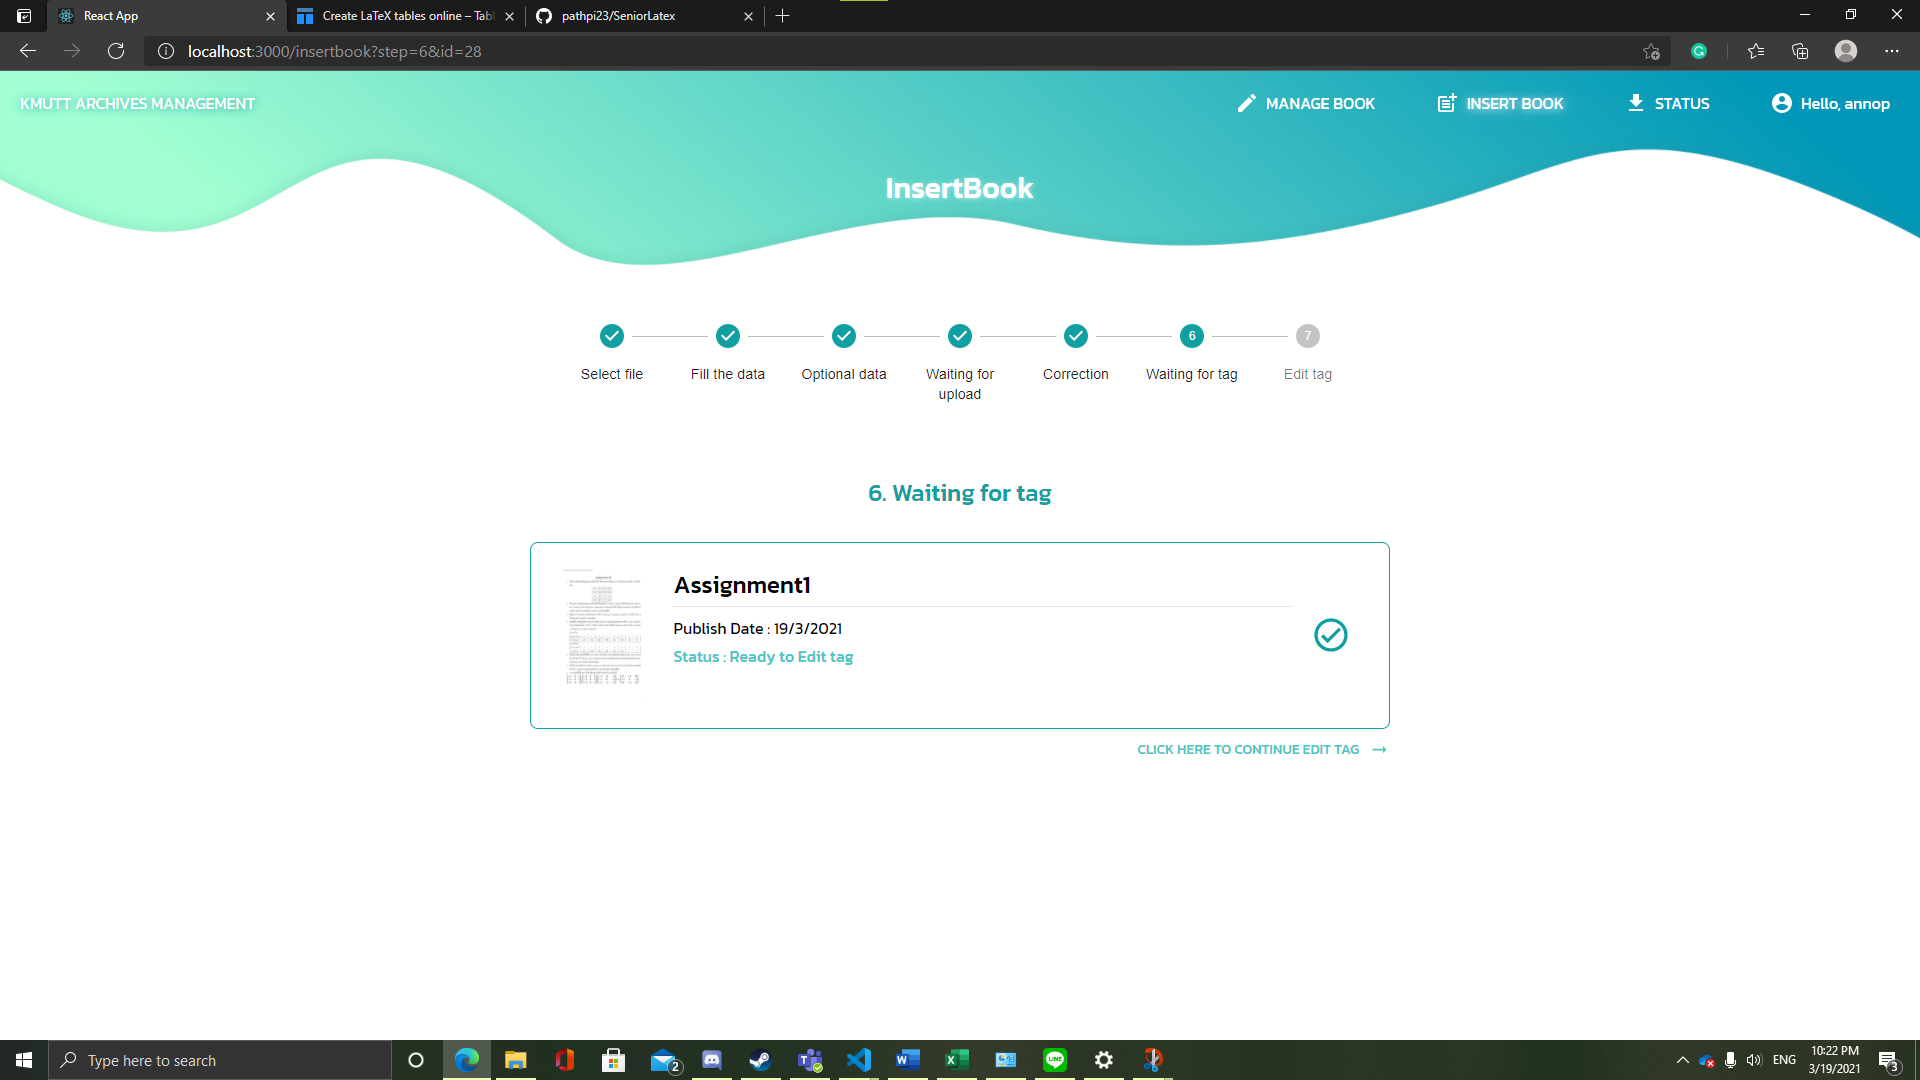
\includegraphics[scale=0.2]{webcheckout}
    \caption{ภาพแสดงขั้นตอนการเพิ่มหนังสือเข้าสู่ระบบขั้นการสร้างคำสำคัญ}\label{fig:webcheckout}
\end{figure}
ในส่วนนี้จะเป็นผลลัพธ์การดำเนินการของการเพิ่มข้อมูลหนังสือ จะมีคำของแต่ละหน้าพร้อมรูปภาพประกอบเพื่อให้ผู้ใช้งานได้ตรวจสอบคำเพิ่มและแก้ไขคำได้อย่างอิสระก่อนจะนำคำเหล่านี้เข้าสู่ระบบและในส่วนนี้ถ้ายืนยันการแก้ไขแล้วจะไม่สามารถมาแก้ไขคำในหนังสือเล่มนี้ในระบบได้อีกโดยถ้ายืนยันแล้วระบบจะทำการเพิ่มคำเหล่านี้เข้าสู่ระบบและทำการคำนวนคะแนน TF/IDF ของคำเหล่านี้ก่อนจะสร้าง tag ของหนังสือเล่มนี้ให้อัตโนมัติ

\subsubsection{การตรวจสอบแก้ไข tag}
\begin{figure}[H]
    \centering
    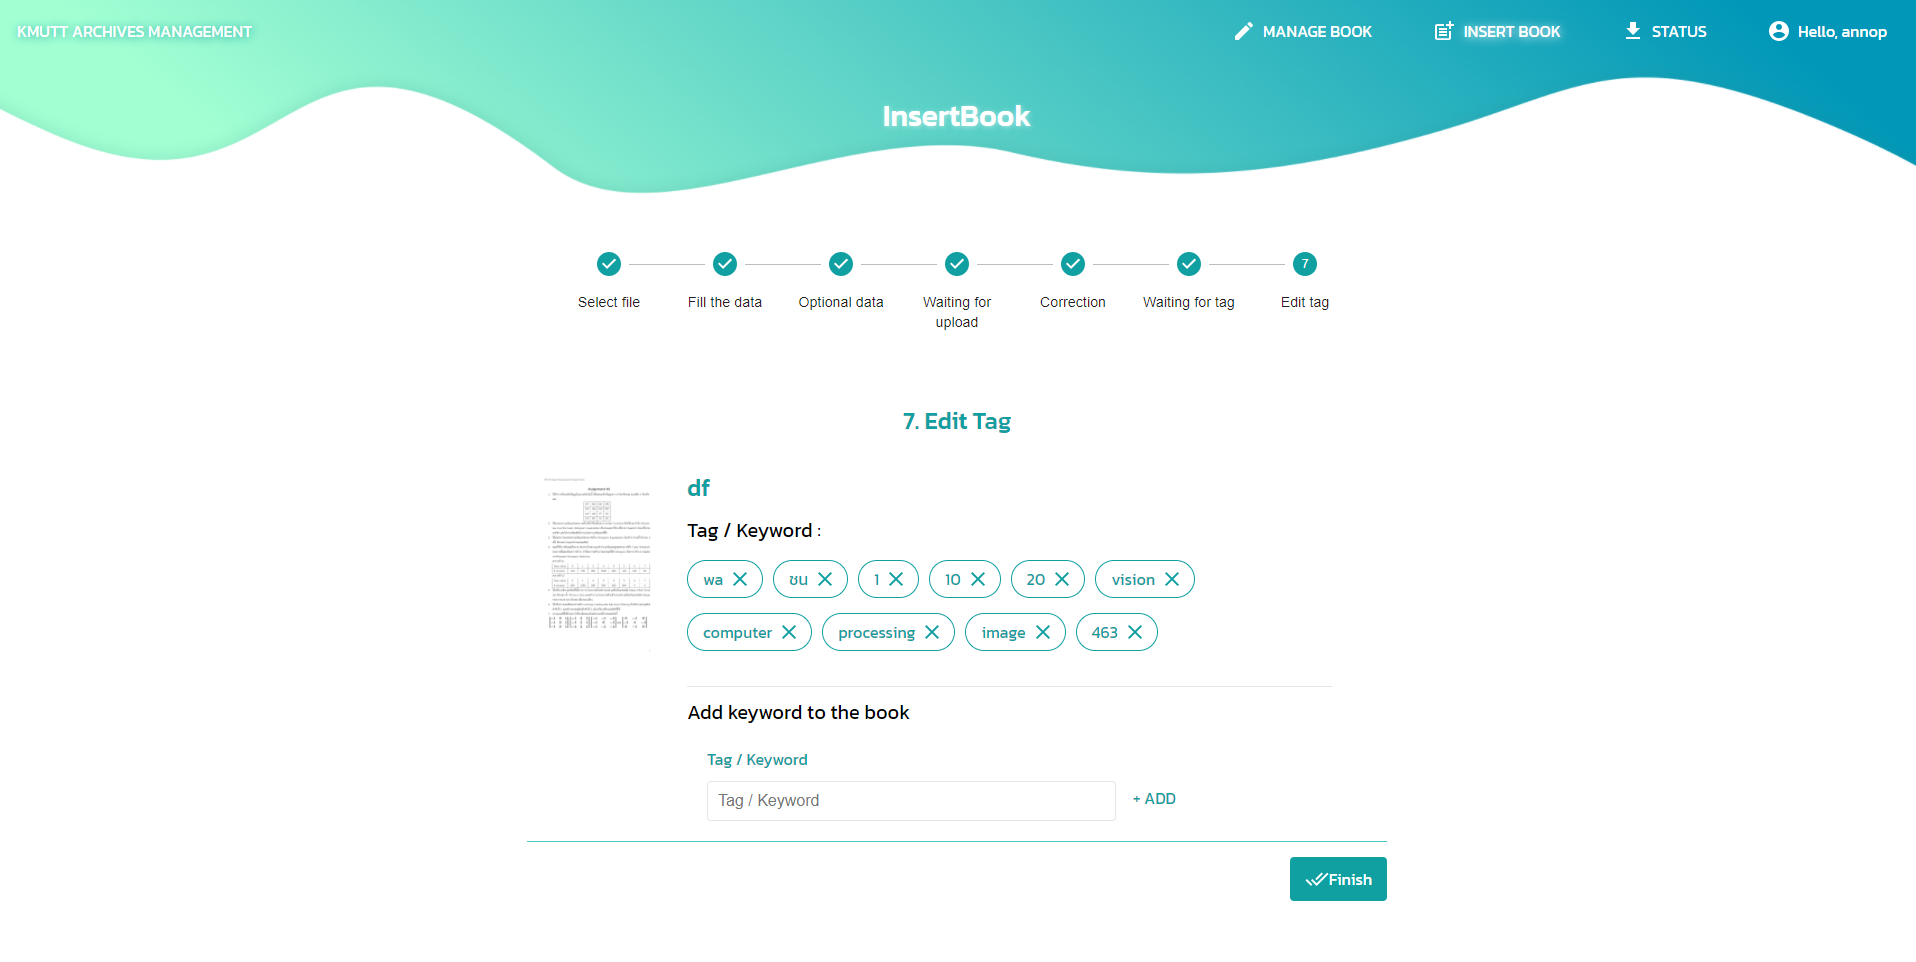
\includegraphics[scale=0.2]{webtag}
    \caption{ภาพแสดงขั้นตอนการเพิ่มหนังสือเข้าสู่ระบบขั้นการแก้ไขคำสำคัญ}\label{fig:webtag}
\end{figure}
ในส่วนนี้จะเป็นผลลัพธ์ของการแก้ไขและตรวจสอบคำก่อนนำเข้าสู่ระบบโดยผู้ใช้งานได้ tag ที่ทางระบบทำขึ้นอัตโนมัติเพื่อให้ผู้ใช้งานได้ตรวจสอบเพิ่มลด tag ก่อนจะยืนยันเพิ่มเข้าสู่ระบบ
\subsection{การแสดงสถานะการเพิ่มหนังสือ}
\begin{figure}[H]
    \centering
    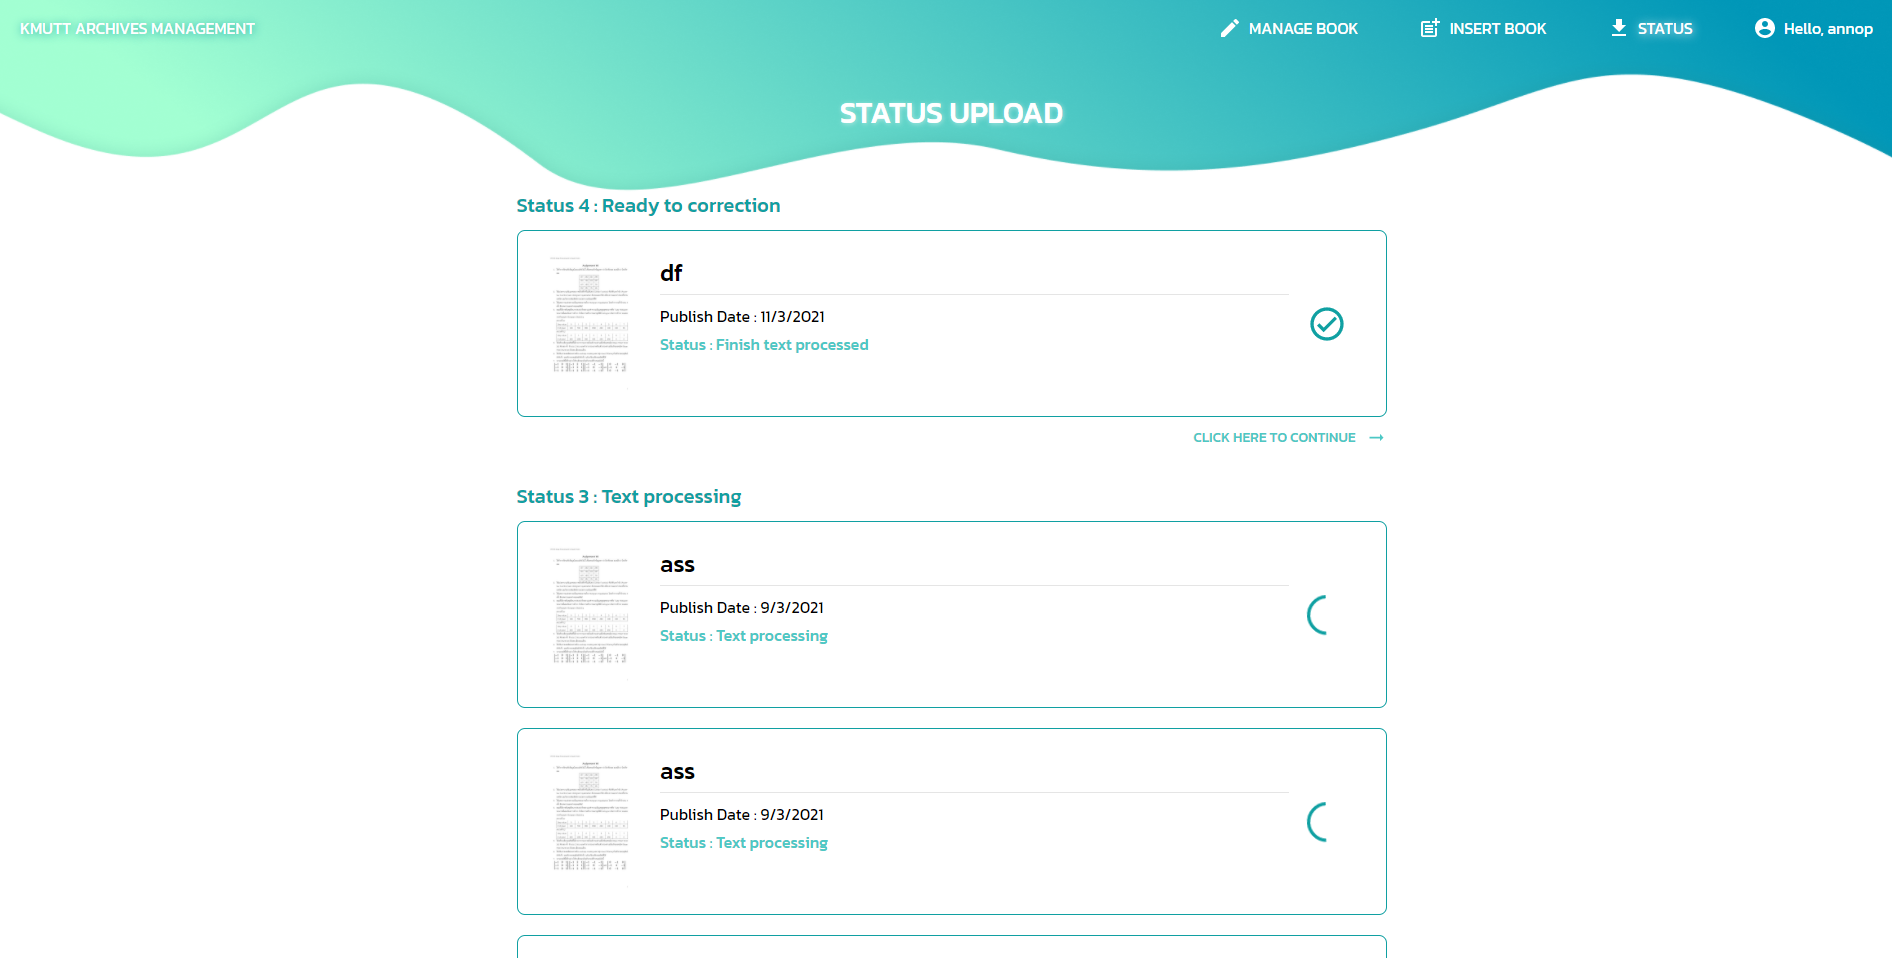
\includegraphics[scale=0.2]{webstatus}
    \caption{ภาพแสดงสถานะของการเพิ่มข้อมูลเข้าสู่ระบบ}\label{fig:webstatus}
\end{figure}

\subsection{การแสดงการค้นหาหนังสือ}
\begin{figure}[H]
    \centering
    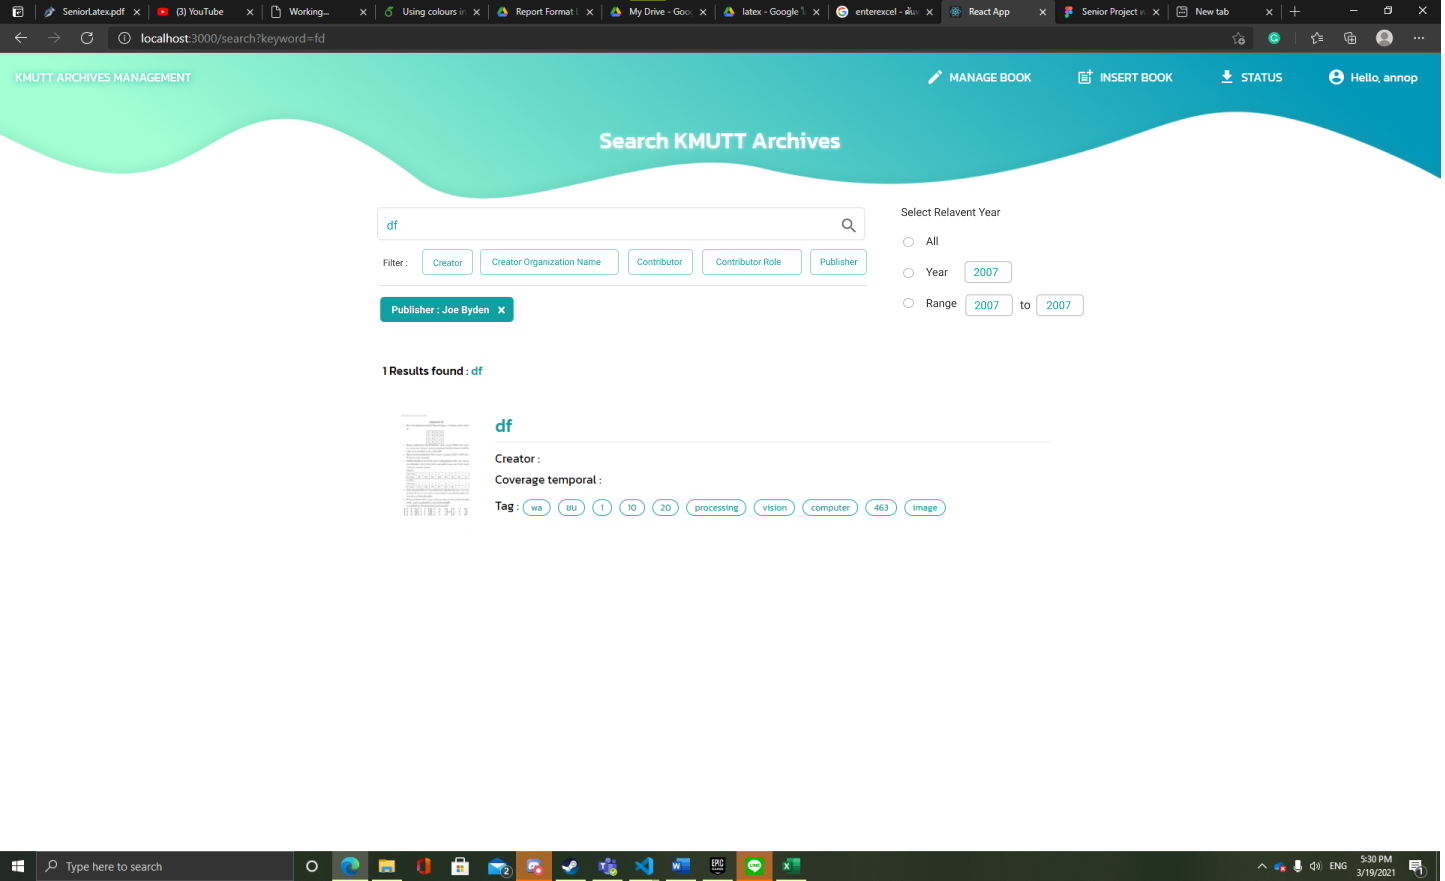
\includegraphics[scale=0.2]{websearch}
    \caption{ภาพแสดงหน้าการค้นหา}\label{fig:websearch}
\end{figure}

\subsection{การแสดงข้อมูลหนังสือ}
\begin{figure}[H]
    \centering
    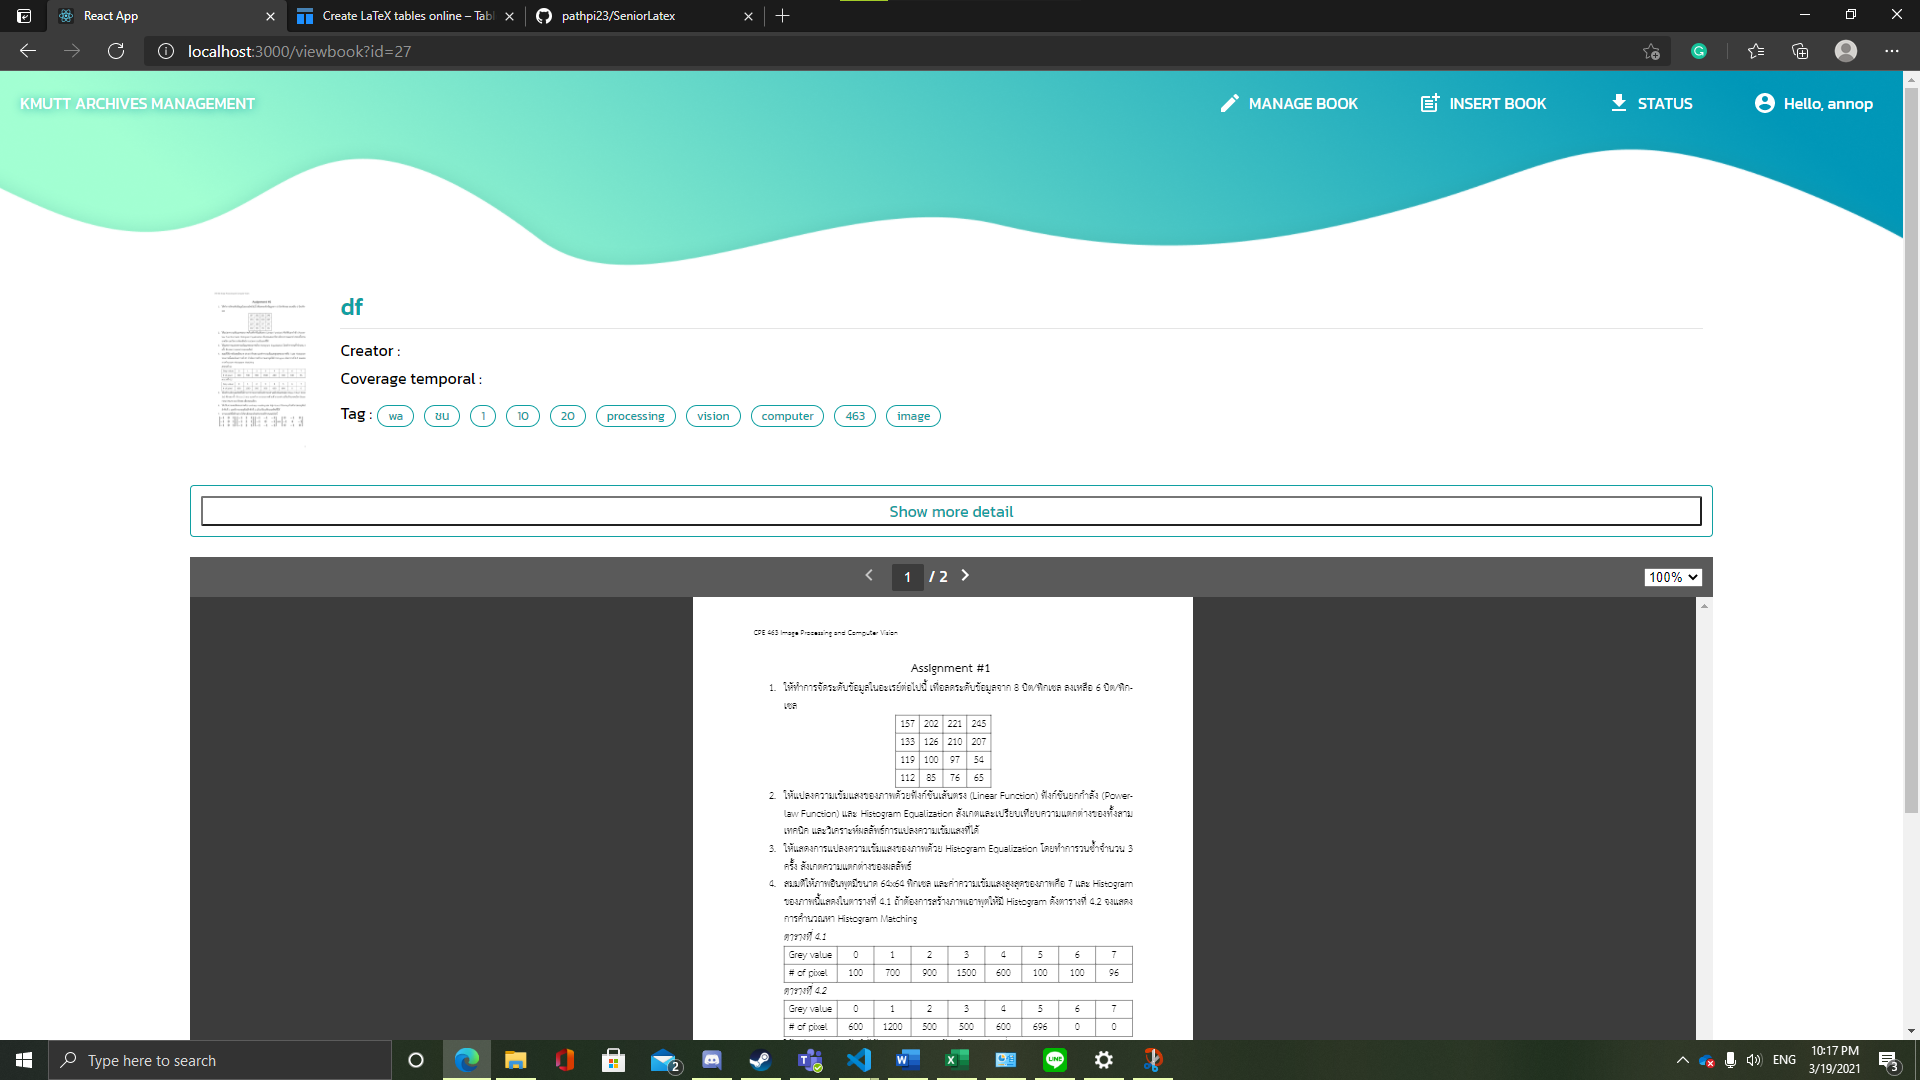
\includegraphics[scale=0.2]{webview}
    \caption{ภาพแสดงหน้าแสดงหนังสือ}\label{fig:webview}
\end{figure}
จะเป็นการแสดงข้อมูลของหนังสือที่อยู่ภายในระบบที่ผู้ใช้งานกรอกเข้ามาในระบบพร้อมทั้งแสดง PDF ที่ถูกอัพโหลดขึ้นมา

\begin{figure}[H]
    \centering
    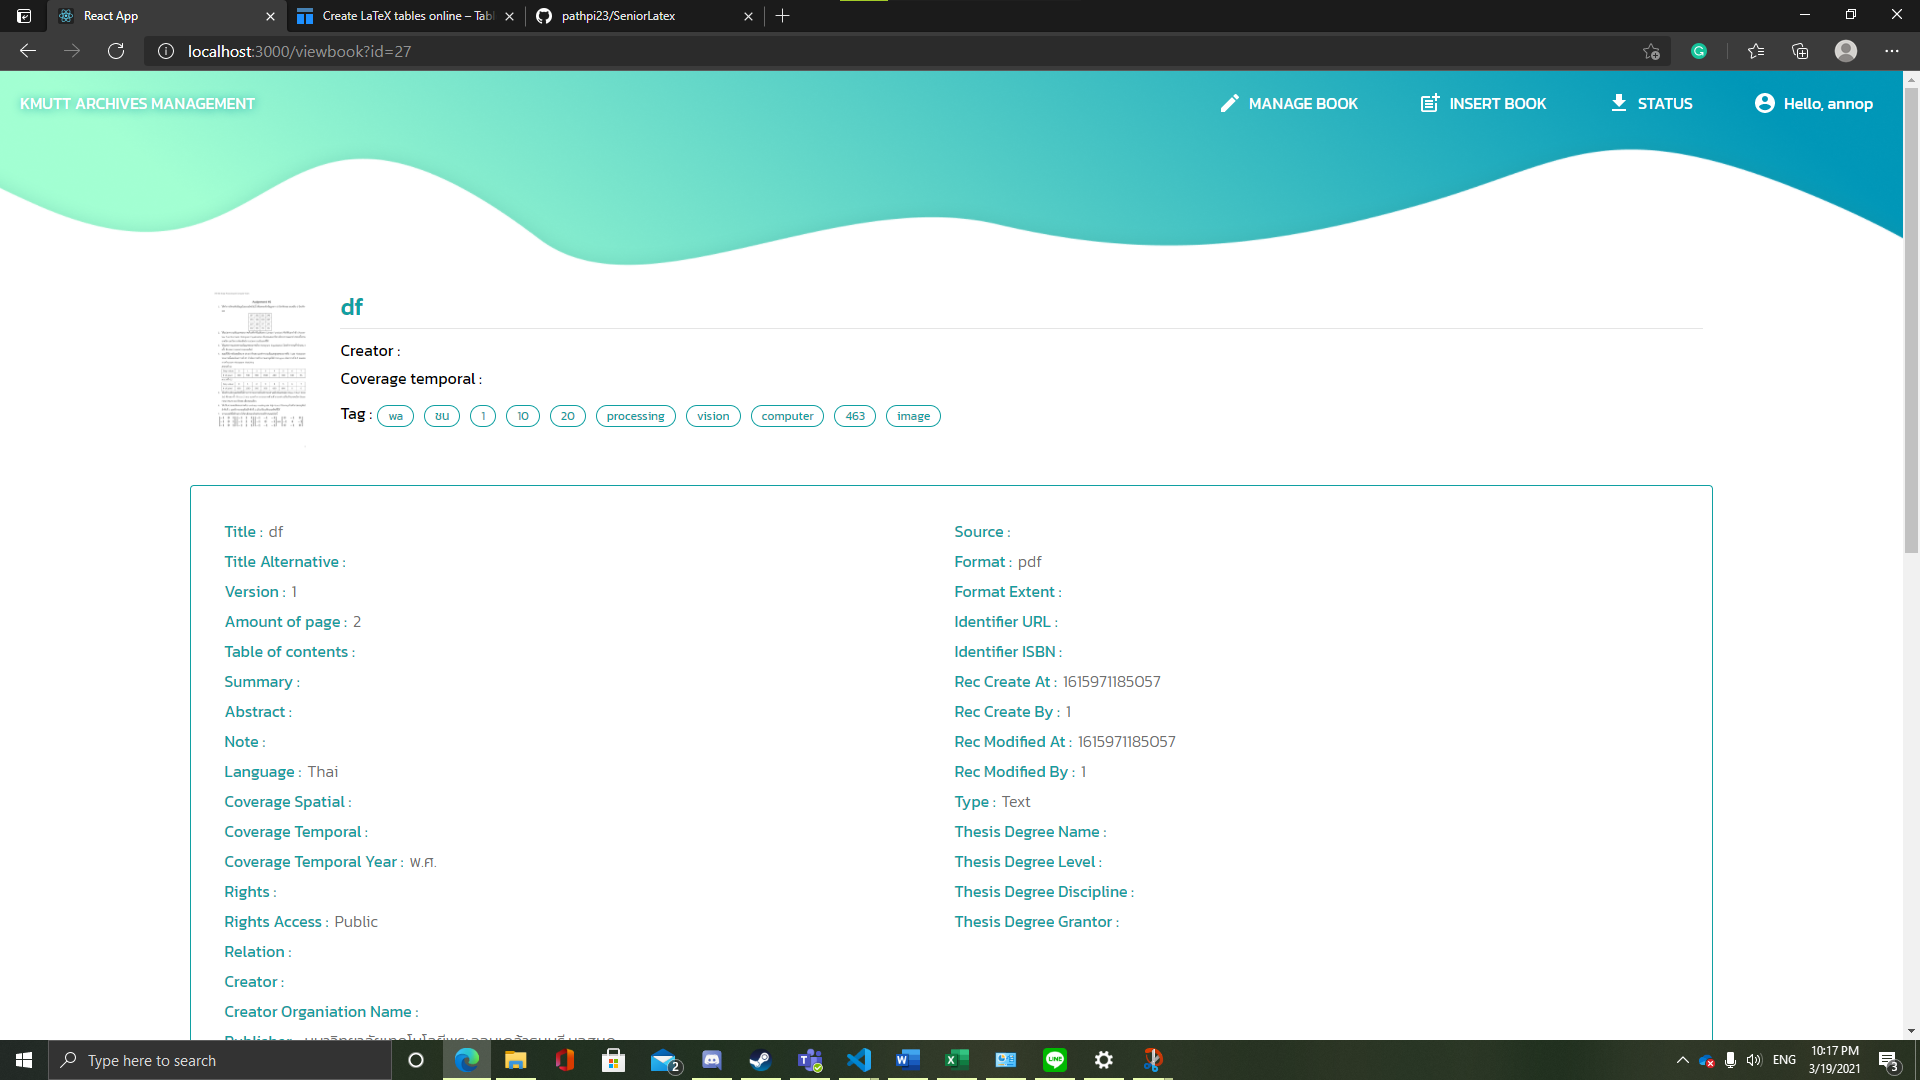
\includegraphics[scale=0.2]{webview2}
    \caption{ภาพแสดงข้อมูลของหนังสือ}\label{fig:webview2}
\end{figure}

\subsection{การแสดงการแก้ไขข้อมูลของหนังสือ}

\begin{figure}[H]
    \centering
    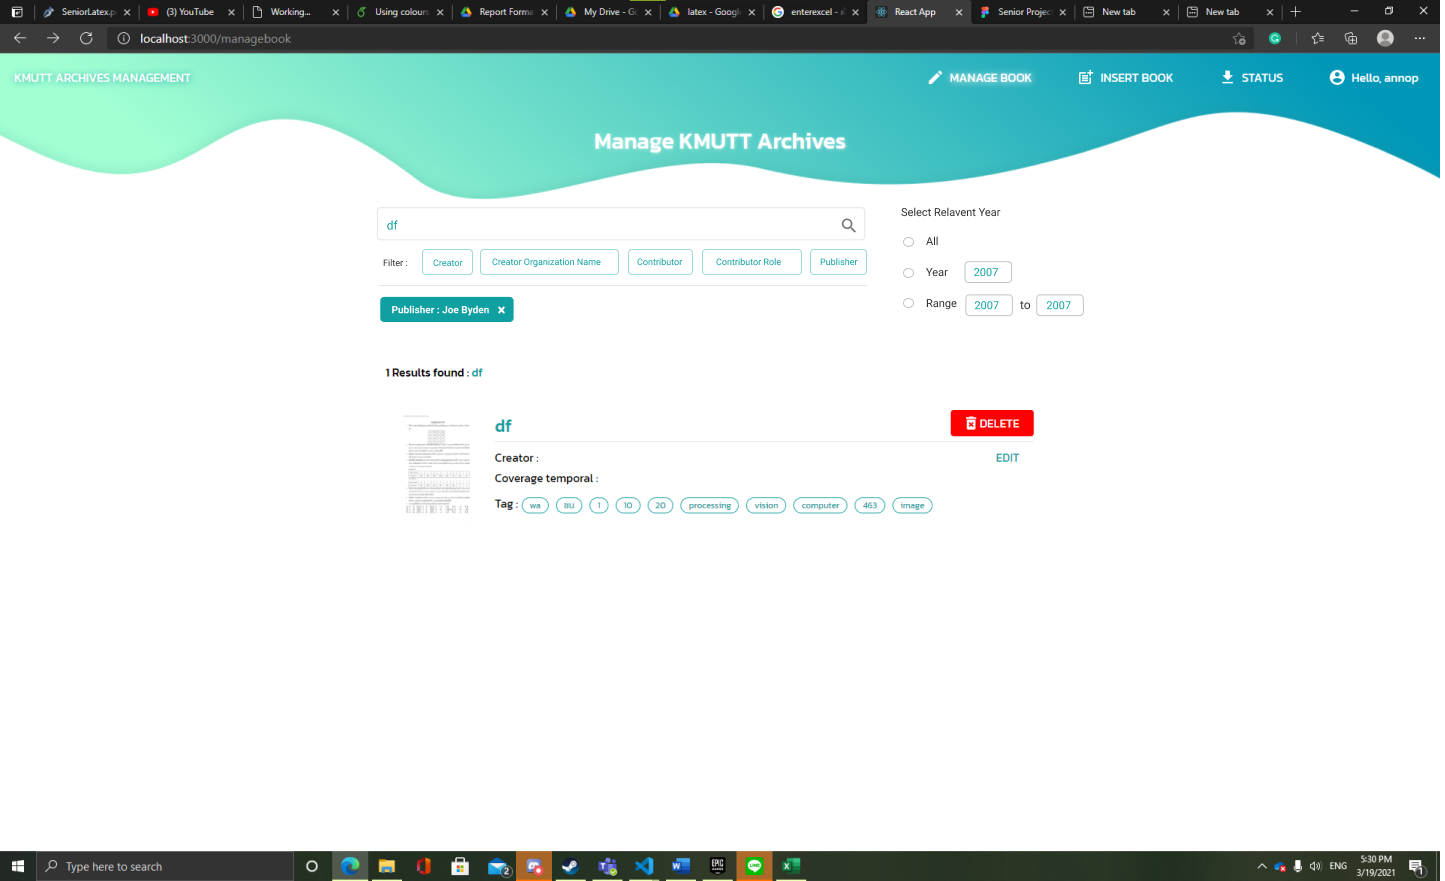
\includegraphics[scale=0.2]{webman}
    \caption{ภาพแสดงหน้าการค้นหาในหน้าการจัดการหนังสือ}\label{fig:webman}
\end{figure}

\begin{figure}[H]
    \centering
    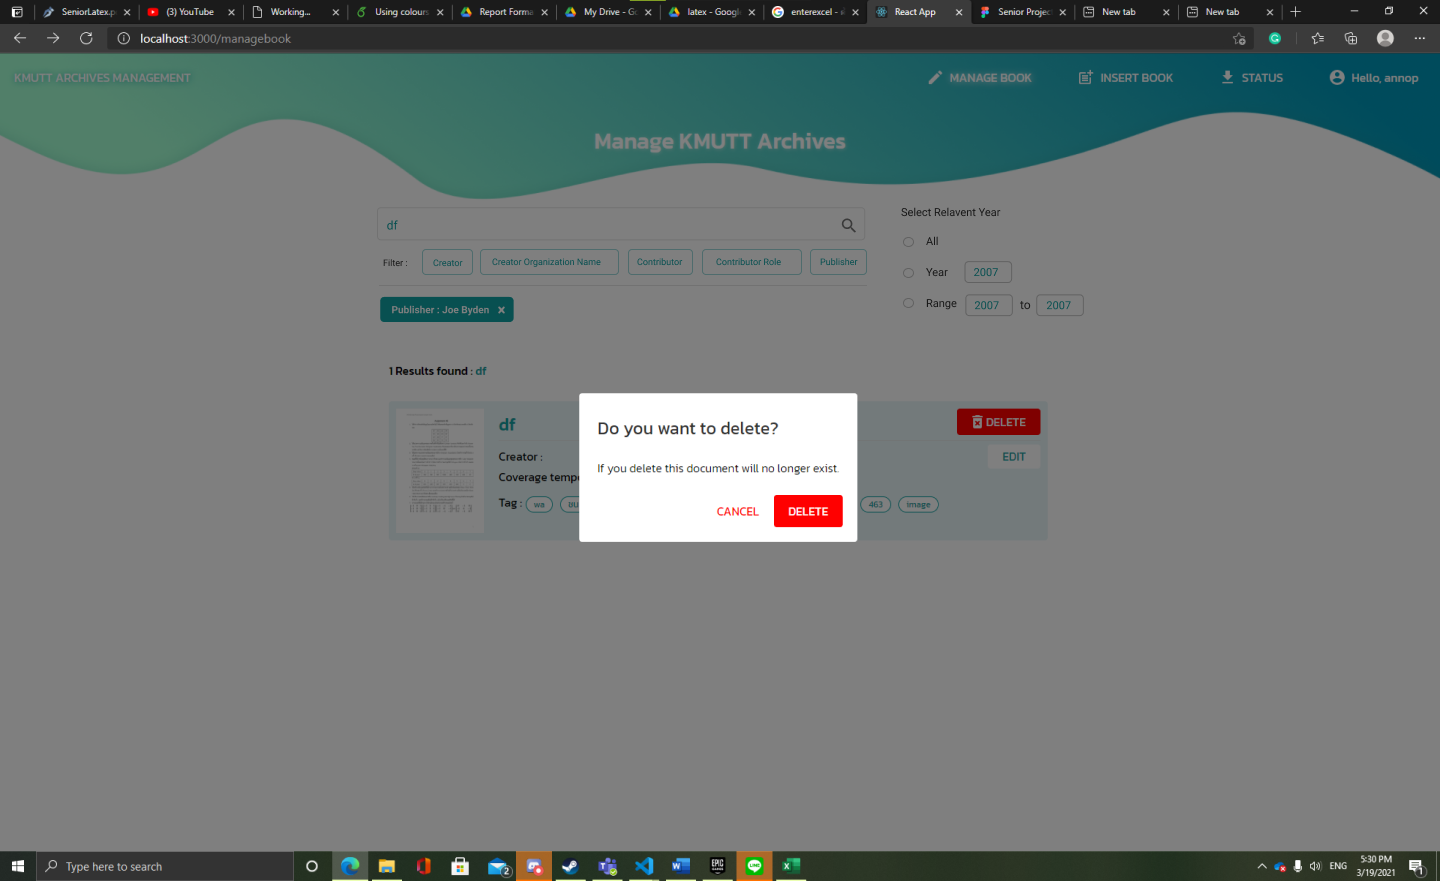
\includegraphics[scale=0.2]{webdel}
    \caption{ภาพแสดงหน้าการลบหนังสือ]}\label{fig:webdel}
\end{figure}

\begin{figure}[H]
    \centering
    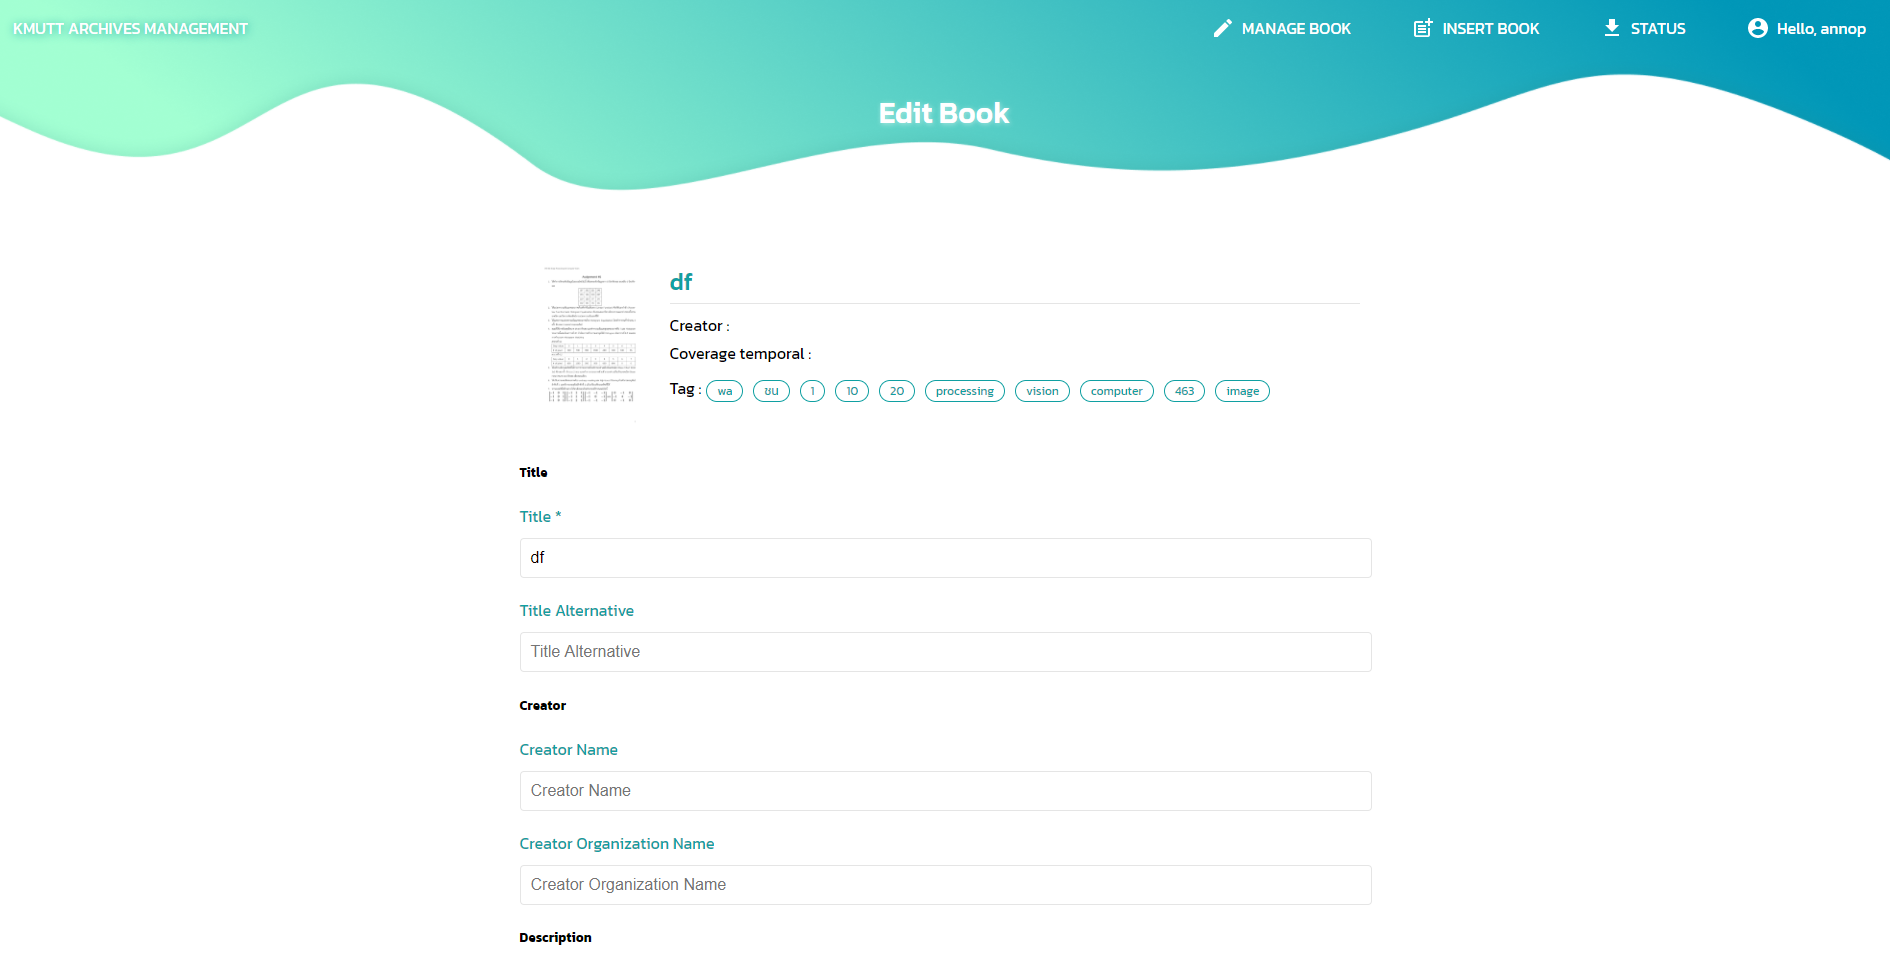
\includegraphics[scale=0.2]{webman1}
    \caption{ภาพแสดงหน้าการแก้ไขข้อมูลขั้นที่ 1}\label{fig:webman1}
\end{figure}

\begin{figure}[H]
    \centering
    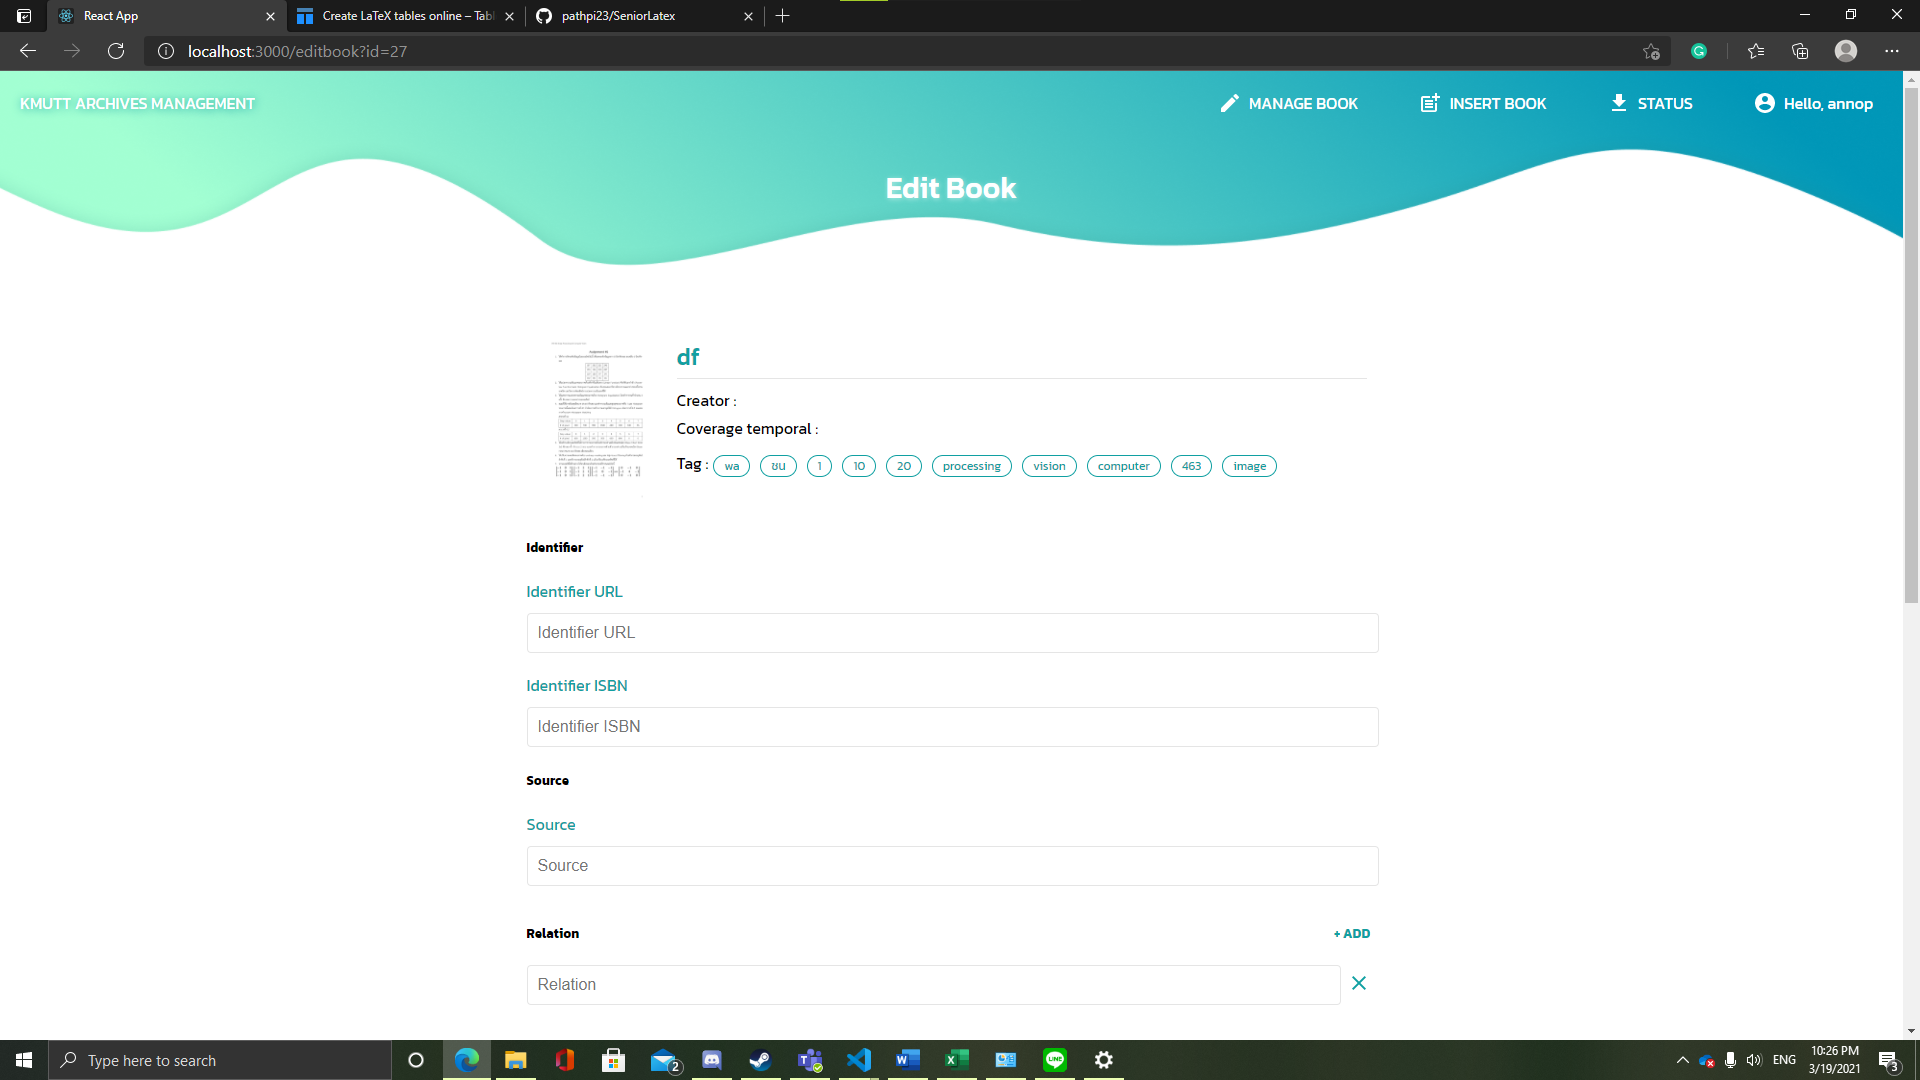
\includegraphics[scale=0.2]{webman3}
    \caption{ภาพแสดงหน้าการแก้ไขข้อมูลขั้นที่ 3}\label{fig:webman2}
\end{figure}

\begin{figure}[H]
    \centering
    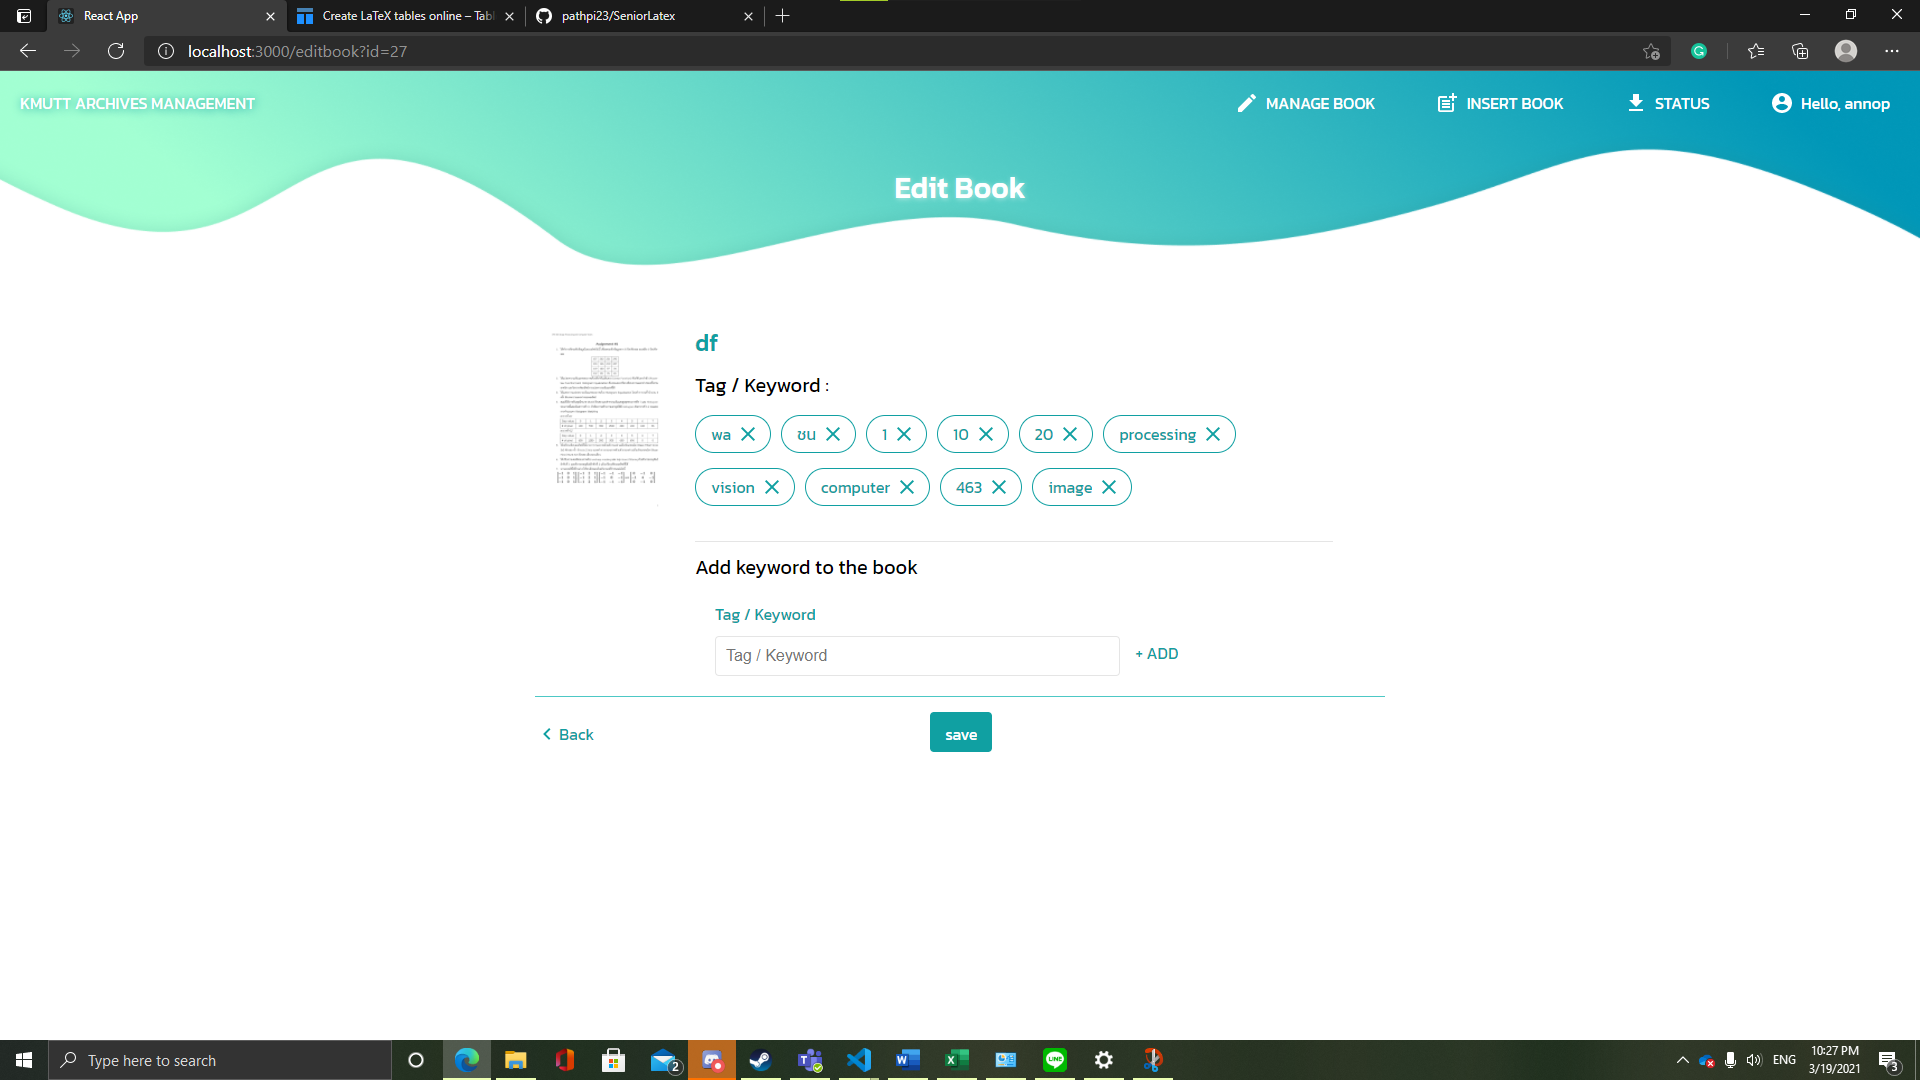
\includegraphics[scale=0.2]{webman4}
    \caption{ภาพแสดงหน้าการแก้ไขคำสำคัญ}\label{fig:webman4}
\end{figure}

การแก้ไขข้อมูลจะแก้ได้ต่อเมื่อเพิ่มข้อมูลหนังสือเสร็จสิ้นแล้วโดยที่จะสามารถแก้ไขข้อมูลในส่วนของข้อมูลหนังสือและ tag ได้เหมือนกันกับการเพิ่มหนังสือโดยเมื่อแก้ไขเสร็จสิ้นแล้วยืนยันระบบจะทำการบันทึกข้อมูลใหม่ให้ทันที